
% LaTeX Beamer file automatically generated from DocOnce
% https://github.com/doconce/doconce

%-------------------- begin beamer-specific preamble ----------------------

\documentclass{beamer}

\usetheme{red_plain}
\usecolortheme{default}

% turn off the almost invisible, yet disturbing, navigation symbols:
\setbeamertemplate{navigation symbols}{}

% Examples on customization:
%\usecolortheme[named=RawSienna]{structure}
%\usetheme[height=7mm]{Rochester}
%\setbeamerfont{frametitle}{family=\rmfamily,shape=\itshape}
%\setbeamertemplate{items}[ball]
%\setbeamertemplate{blocks}[rounded][shadow=true]
%\useoutertheme{infolines}
%
%\usefonttheme{}
%\useinntertheme{}
%
%\setbeameroption{show notes}
%\setbeameroption{show notes on second screen=right}

% fine for B/W printing:
%\usecolortheme{seahorse}

\usepackage{pgf}
\usepackage{graphicx}
\usepackage{epsfig}
\usepackage{relsize}

\usepackage{fancybox}  % make sure fancybox is loaded before fancyvrb

\usepackage{fancyvrb}
\usepackage{minted} % requires pygments and latex -shell-escape filename
%\usepackage{anslistings}
%\usepackage{listingsutf8}

\usepackage{amsmath,amssymb,bm}
%\usepackage[latin1]{inputenc}
\usepackage[T1]{fontenc}
\usepackage[utf8]{inputenc}
\usepackage{colortbl}
\usepackage[english]{babel}
\usepackage{tikz}
\usepackage{framed}
% Use some nice templates
\beamertemplatetransparentcovereddynamic

% --- begin table of contents based on sections ---
% Delete this, if you do not want the table of contents to pop up at
% the beginning of each section:
% (Only section headings can enter the table of contents in Beamer
% slides generated from DocOnce source, while subsections are used
% for the title in ordinary slides.)
\AtBeginSection[]
{
  \begin{frame}<beamer>[plain]
  \frametitle{}
  %\frametitle{Outline}
  \tableofcontents[currentsection]
  \end{frame}
}
% --- end table of contents based on sections ---

% If you wish to uncover everything in a step-wise fashion, uncomment
% the following command:

%\beamerdefaultoverlayspecification{<+->}

\newcommand{\shortinlinecomment}[3]{\note{\textbf{#1}: #2}}
\newcommand{\longinlinecomment}[3]{\shortinlinecomment{#1}{#2}{#3}}

\definecolor{linkcolor}{rgb}{0,0,0.4}
\hypersetup{
    colorlinks=true,
    linkcolor=linkcolor,
    urlcolor=linkcolor,
    pdfmenubar=true,
    pdftoolbar=true,
    bookmarksdepth=3
    }
\setlength{\parskip}{0pt}  % {1em}

\newenvironment{doconceexercise}{}{}
\newcounter{doconceexercisecounter}
\newenvironment{doconce:movie}{}{}
\newcounter{doconce:movie:counter}

\newcommand{\subex}[1]{\noindent\textbf{#1}}  % for subexercises: a), b), etc

%-------------------- end beamer-specific preamble ----------------------

% Add user's preamble




% insert custom LaTeX commands...

\raggedbottom
\makeindex

%-------------------- end preamble ----------------------

\begin{document}

% matching end for #ifdef PREAMBLE

\newcommand{\exercisesection}[1]{\subsection*{#1}}



% ------------------- main content ----------------------



% ----------------- title -------------------------

\title{Machine Learning for Nuclear Physics and Many-body Physics}

% ----------------- author(s) -------------------------

\author{Morten Hjorth-Jensen\inst{1}}
\institute{Department of Physics and Center for Computing in Science Education, University of Oslo, Norway\inst{1}}
% ----------------- end author(s) -------------------------

\date{Center for Computational Sciences, University of Tsukuba, February 20, 2026
% <optional titlepage figure>
% <optional copyright>
}

\begin{frame}[plain,fragile]
\titlepage
\end{frame}

\begin{frame}[plain,fragile]
\frametitle{What is this talk about?}

\begin{block}{}
The main emphasis is to give you a short and pedestrian introduction to the whys and hows we can use (with several examples) machine learning methods to solve quantum mechanical many-body problemss. And why this could (or should) be of interest. 
\end{block}

\begin{block}{Recent preprint (PPNN submitted) }
Lovato, Carleo, Fore, MHJ, Jane Kim, Rios, Rocco, \textbf{Neural-network quantum states for the nuclear many-body problem}, see \href{{https://arxiv.org/abs/2602.13826}}{\nolinkurl{https://arxiv.org/abs/2602.13826}}
\end{block}
\end{frame}

\begin{frame}[plain,fragile]
\frametitle{Thanks to many}

Jane Kim (ANL), Patrick Cook (MSU), Danny Jammooa (MSU/Riken), Dean
Lee (MSU), Even Nordhagen (UiO), Aleksander Sekkelsten (UiO), Bryce Fore (ANL), Alessandro Lovato
(ANL), Stefano Gandolfi (LANL), Francesco Pederiva (UniTN), Arnau Rios
(Barcelona), and Giuseppe Carleo (EPFL).  Excuses to those I have
omitted/forgotten.
\end{frame}

\begin{frame}[plain,fragile]
\frametitle{AI/ML and some statements you may have heard (and what do they mean?)}

\begin{enumerate}
\item Fei-Fei Li on ImageNet: \textbf{map out the entire world of objects} (\href{{https://cacm.acm.org/news/219702-the-data-that-transformed-ai-research-and-possibly-the-world/fulltext}}{The data that transformed AI research})

\item Russell and Norvig in their popular textbook: \textbf{relevant to any intellectual task; it is truly a universal field} (\href{{http://aima.cs.berkeley.edu/}}{Artificial Intelligence, A modern approach})

\item Woody Bledsoe puts it more bluntly: \textbf{in the long run, AI is the only science} (quoted in Pamilla McCorduck, \href{{https://www.pamelamccorduck.com/machines-who-think}}{Machines who think})
\end{enumerate}

\noindent
If you wish to have a critical read on AI/ML from a societal point of view, see \href{{https://www.katecrawford.net/}}{Kate Crawford's recent text Atlas of AI}.

\textbf{Here: with AI/ML we intend a collection of machine learning methods with an emphasis on statistical learning and data analysis}
\end{frame}

\begin{frame}[plain,fragile]
\frametitle{Qauntum mechanical many-body problems (nuclear example here)}

\vspace{6mm}

% inline figure
\centerline{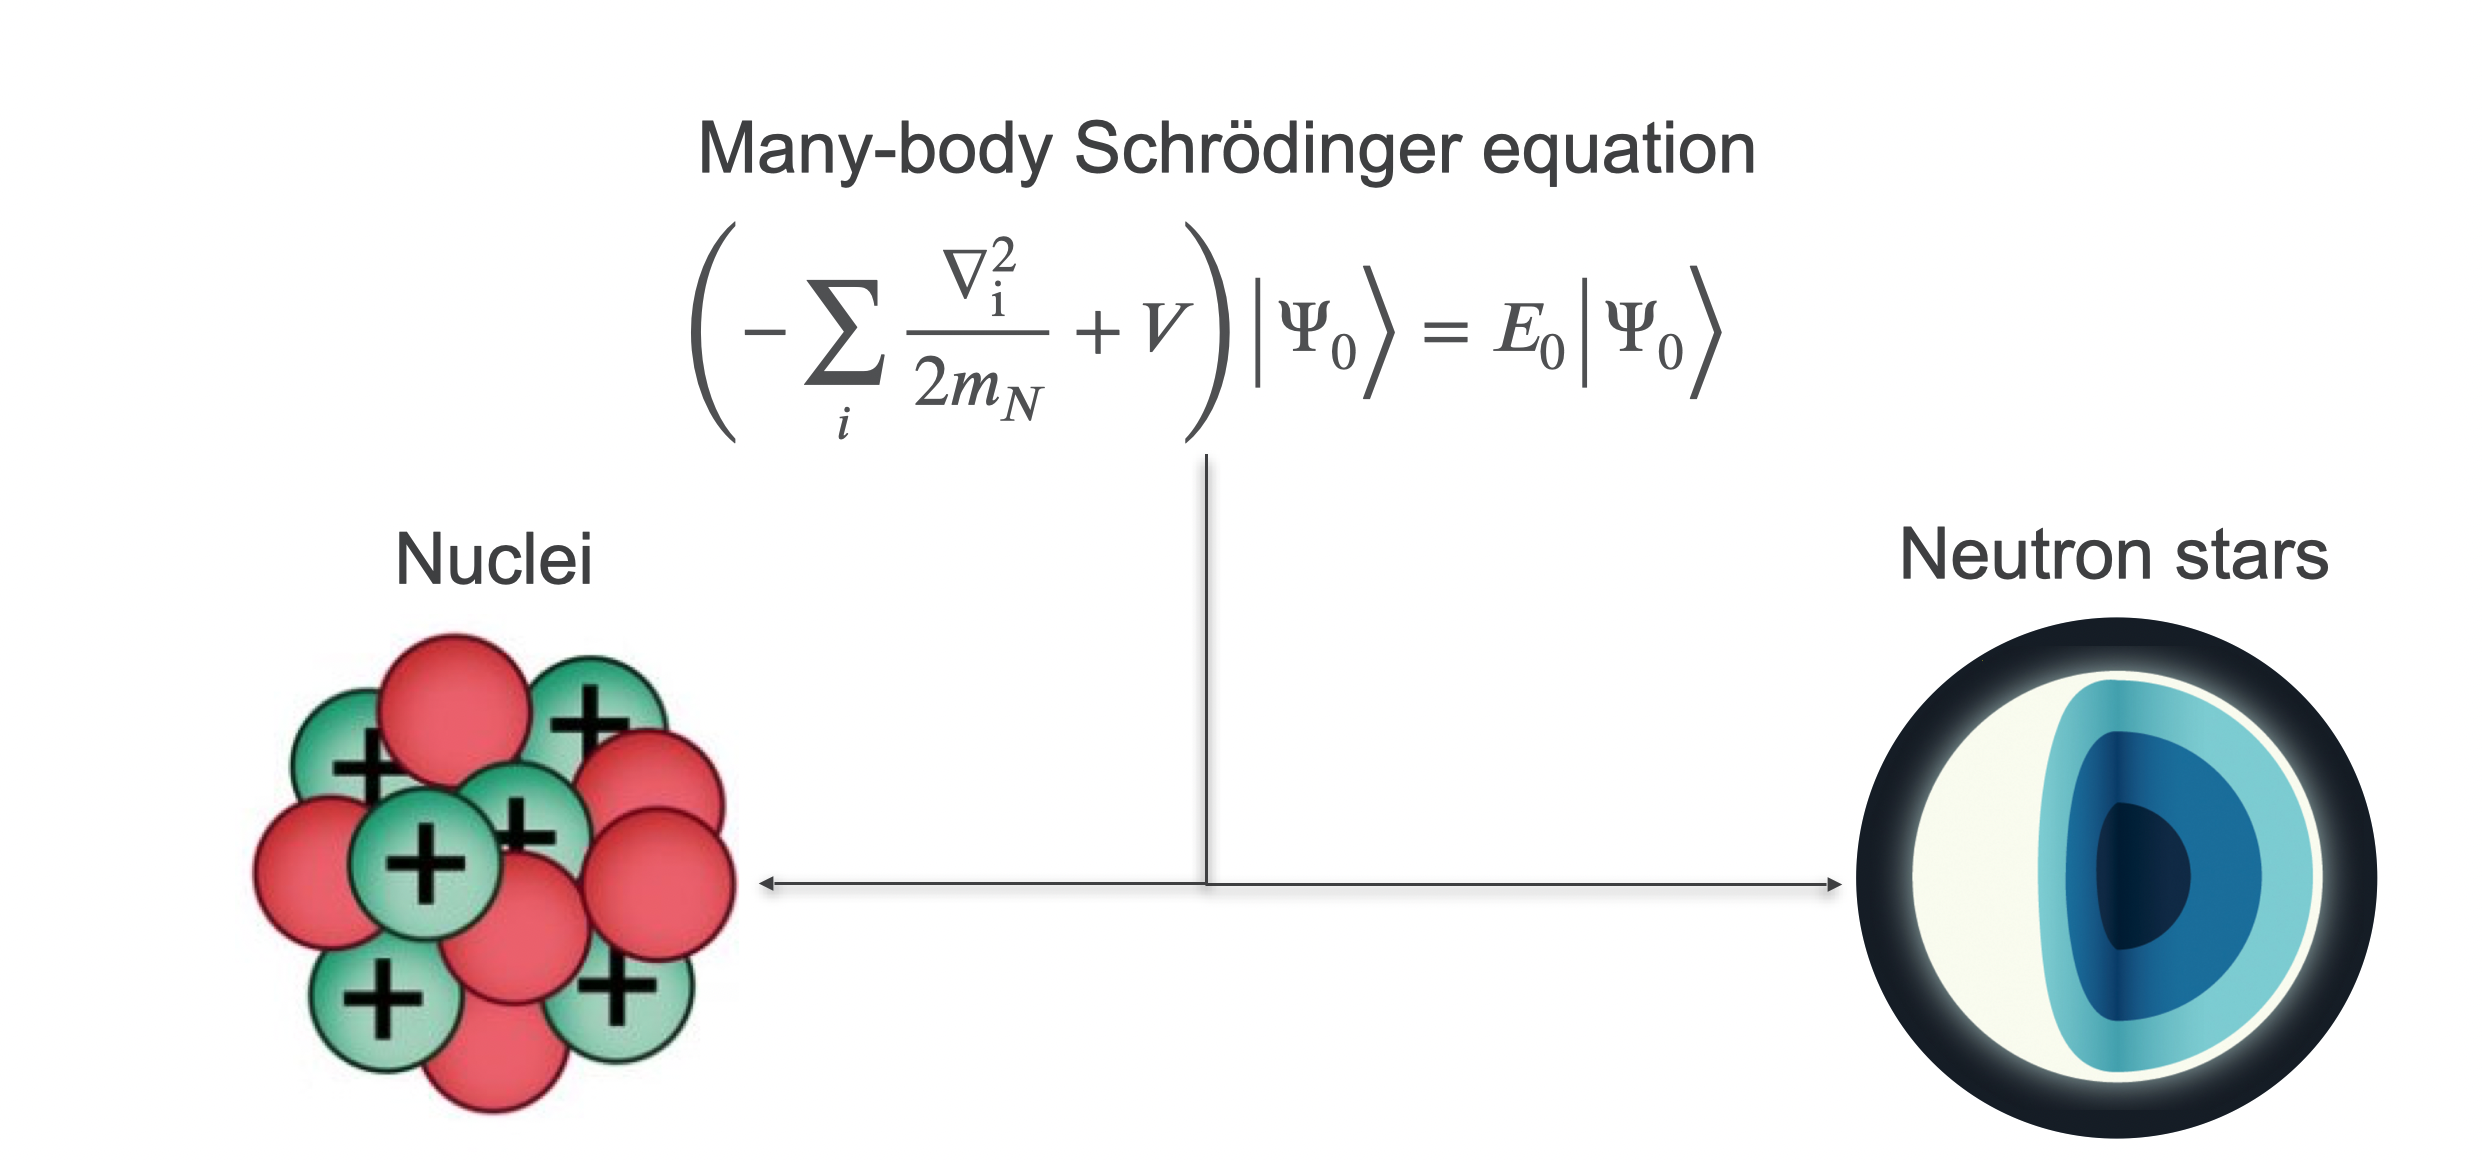
\includegraphics[width=1.1\linewidth]{figures/mbpfig1.png}}

\vspace{6mm}
\end{frame}

\begin{frame}[plain,fragile]
\frametitle{Curse of dimensionality}

\vspace{6mm}

% inline figure
\centerline{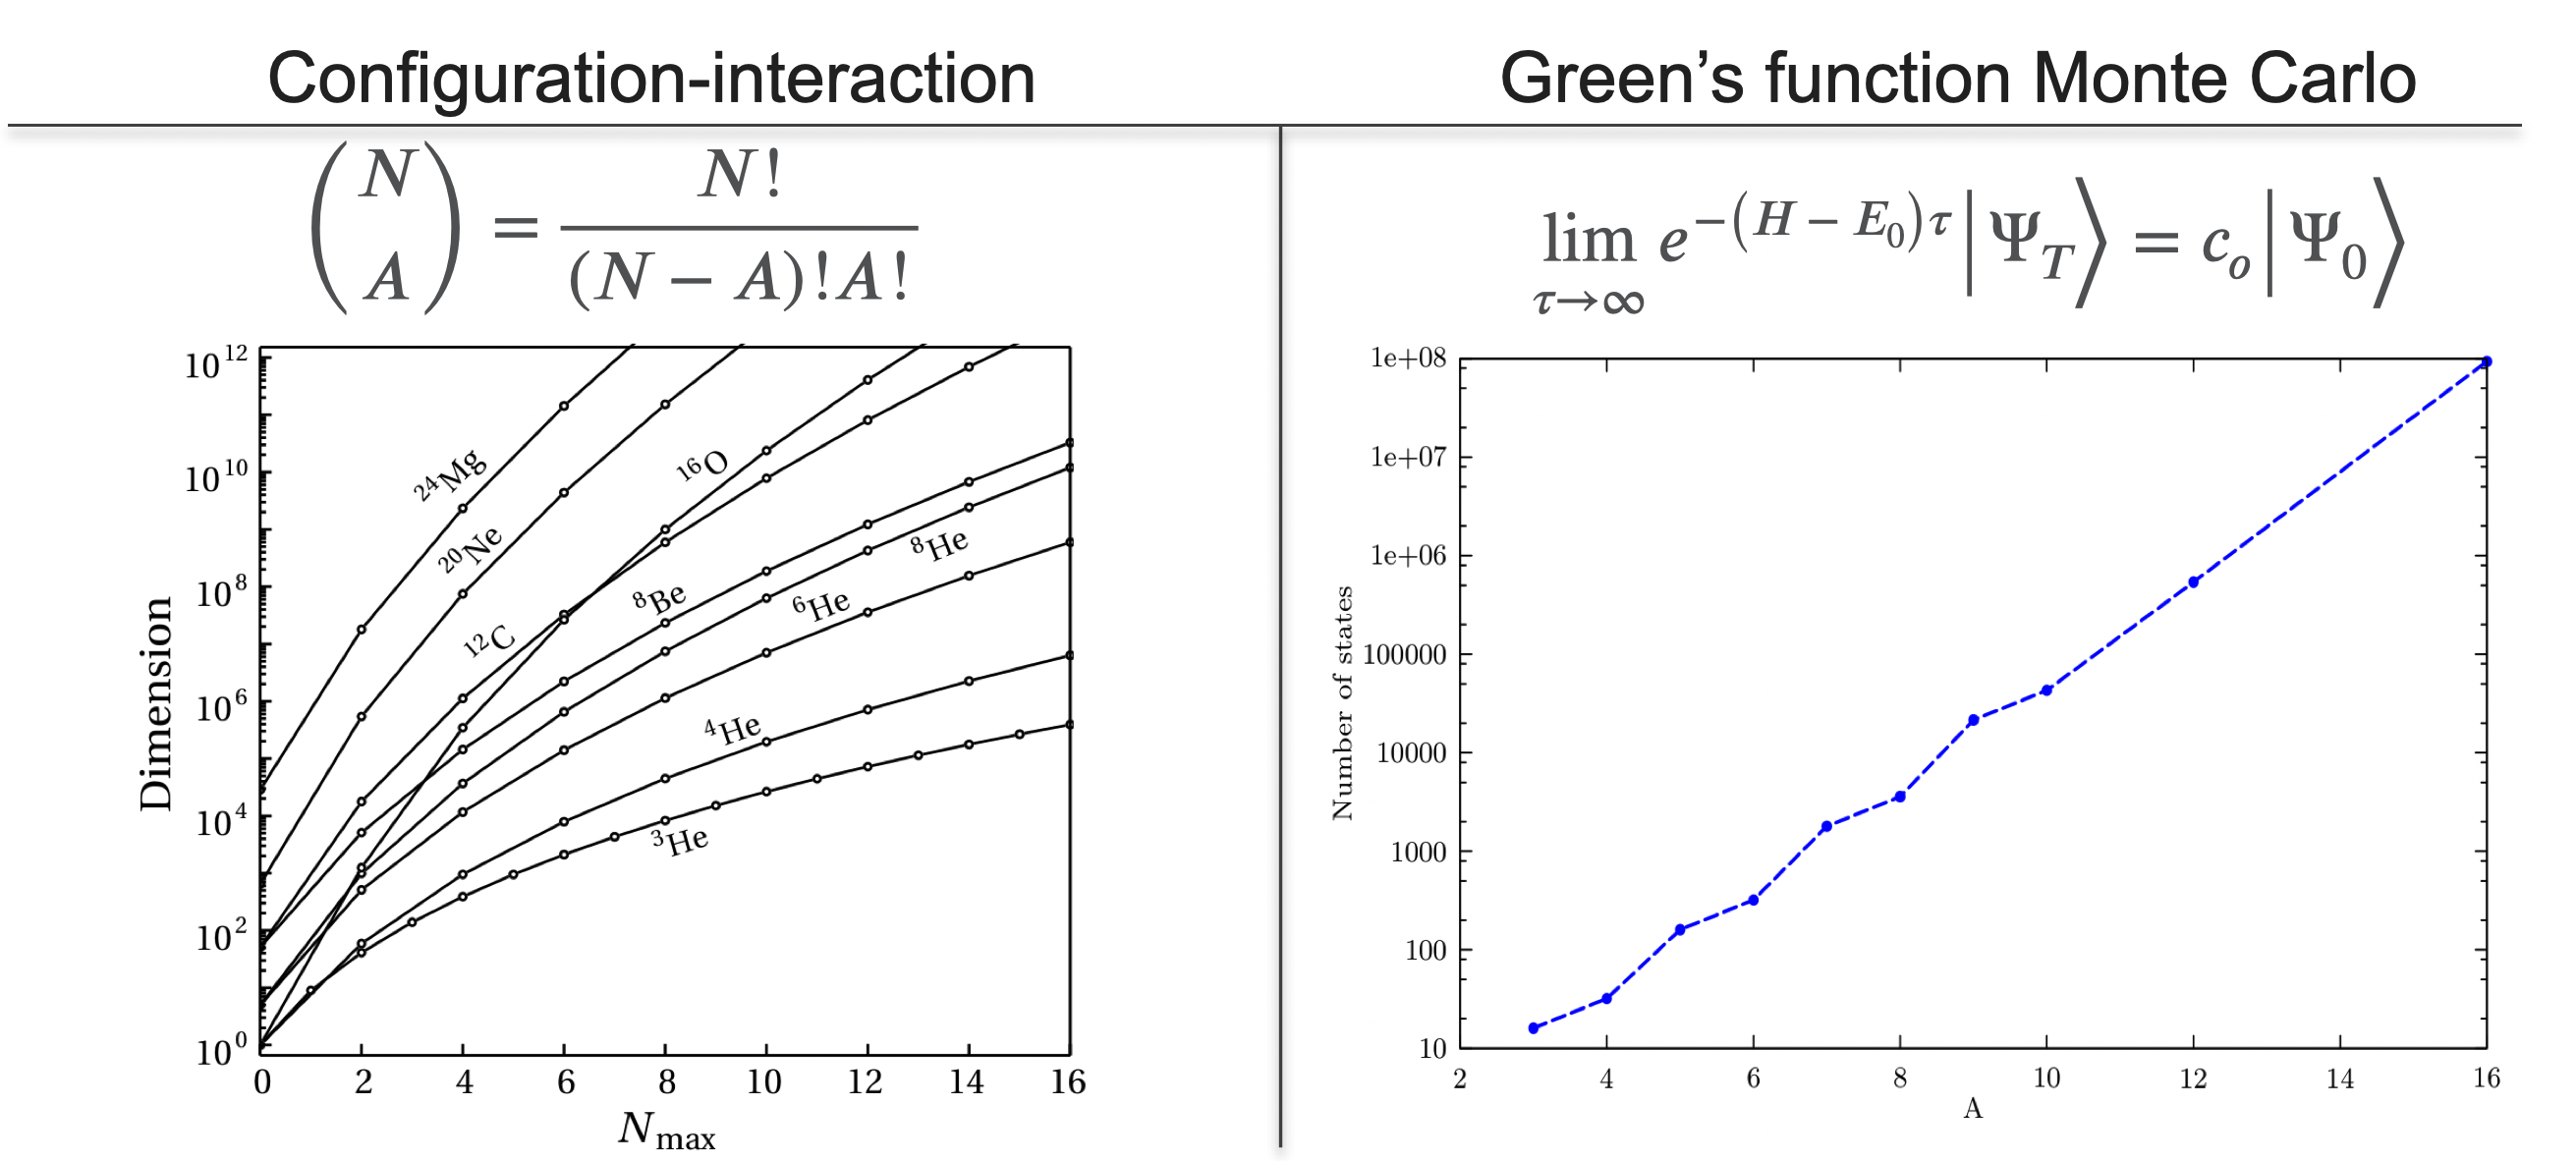
\includegraphics[width=1.0\linewidth]{figures/mbpfig2.png}}

\vspace{6mm}
\end{frame}

\begin{frame}[plain,fragile]
\frametitle{Neural network quantum states}

\begin{block}{Neural networks compactly represent complex high-dimensional functions }
Most quantum states of interest have distinctive features and intrinsic structures

\vspace{6mm}

% inline figure
\centerline{
\includegraphics[width=1.0\linewidth]{figures/mbpfig3.png}}

\vspace{6mm}

\end{block}
\end{frame}

\begin{frame}[plain,fragile]
\frametitle{Machine learning. A simple perspective on the interface between ML and Physics}

\vspace{6mm}

% inline figure
\centerline{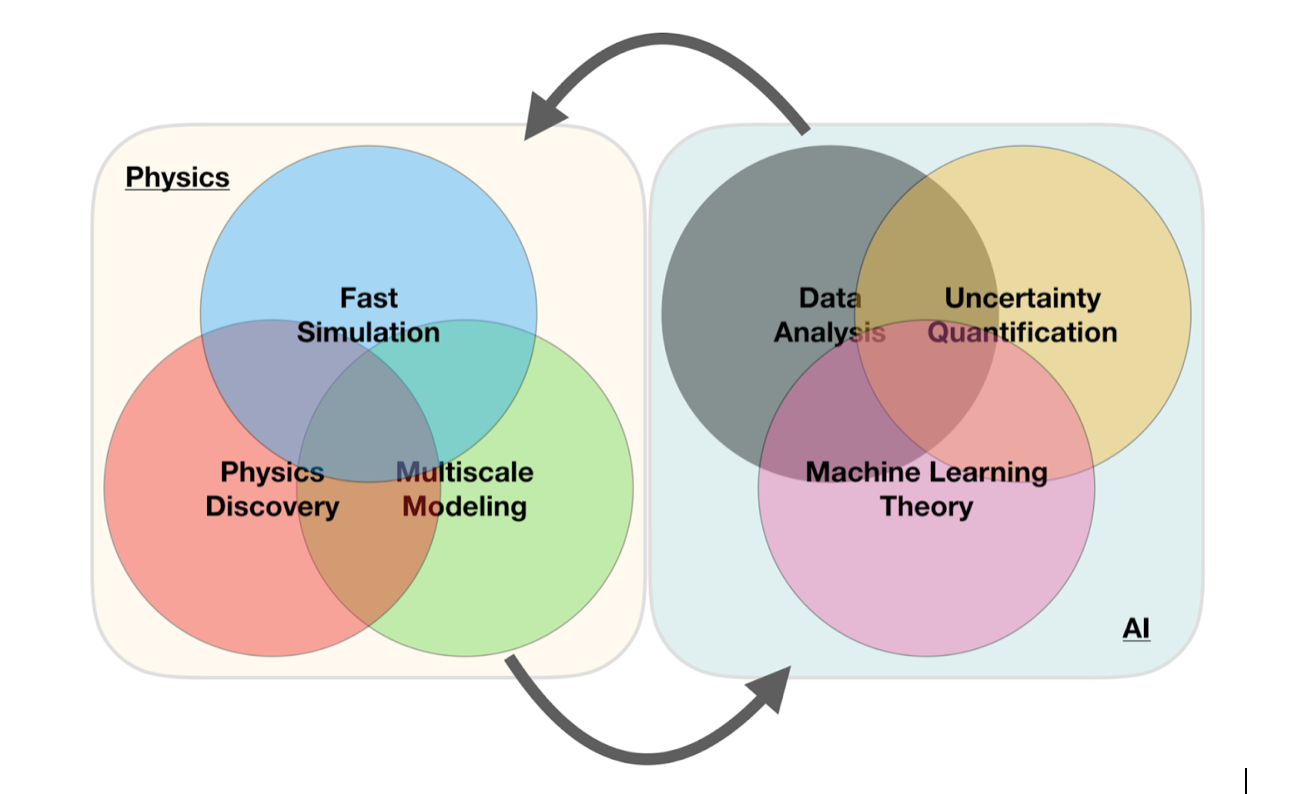
\includegraphics[width=1.0\linewidth]{figures/mlimage.png}}

\vspace{6mm}
\end{frame}

\begin{frame}[plain,fragile]
\frametitle{ML in Nuclear  Physics (or any field, almost)}

\vspace{6mm}

% inline figure
\centerline{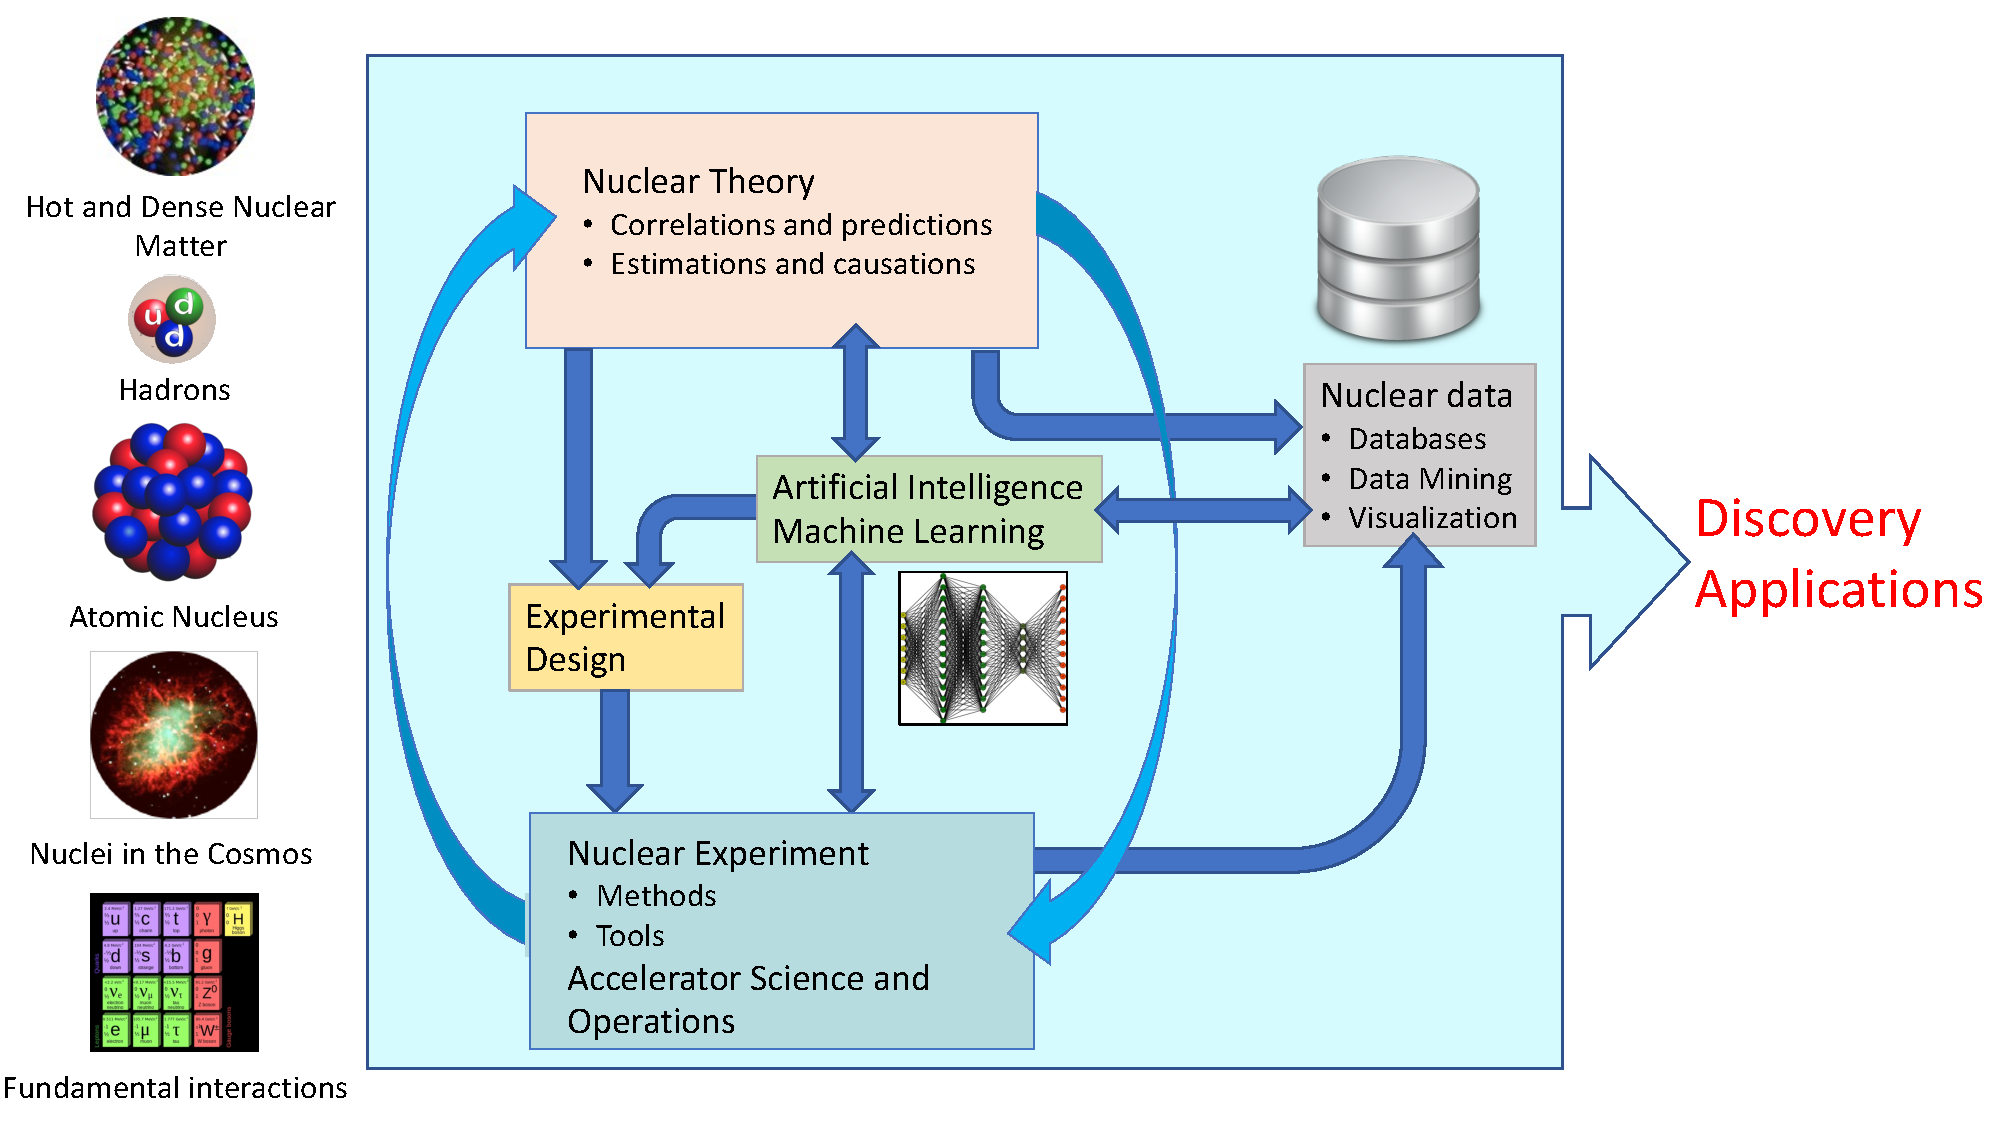
\includegraphics[width=1.0\linewidth]{figures/ML-NP.pdf}}

\vspace{6mm}
\end{frame}

\begin{frame}[plain,fragile]
\frametitle{Types of machine learning}

\begin{block}{}
The approaches to machine learning are many, but are often split into two main categories. 
In \emph{supervised learning} we know the answer to a problem,
and let the computer deduce the logic behind it. On the other hand, \emph{unsupervised learning}
is a method for finding patterns and relationship in data sets without any prior knowledge of the system.

An important  third category is  \emph{reinforcement learning}. This is a paradigm 
of learning inspired by behavioural psychology, where learning is achieved by trial-and-error, 
solely from rewards and punishment.
\end{block}
\end{frame}

\begin{frame}[plain,fragile]
\frametitle{Main categories}

\begin{block}{}
Another way to categorize machine learning tasks is to consider the desired output of a system.
Some of the most common tasks are:

\begin{itemize}
  \item Classification: Outputs are divided into two or more classes. The goal is to   produce a model that assigns inputs into one of these classes. An example is to identify  digits based on pictures of hand-written ones. Classification is typically supervised learning.

  \item Regression: Finding a functional relationship between an input data set and a reference data set.   The goal is to construct a function that maps input data to continuous output values.

  \item Clustering: Data are divided into groups with certain common traits, without knowing the different groups beforehand.  It is thus a form of unsupervised learning.
\end{itemize}

\noindent
\end{block}
\end{frame}

\begin{frame}[plain,fragile]
\frametitle{The plethora  of machine learning algorithms/methods}

\begin{enumerate}
\item Deep learning: Neural Networks (NN), Convolutional NN, Recurrent NN, Boltzmann machines, autoencoders and variational autoencoders  and generative adversarial networks, stable diffusion and many more generative models

\item Bayesian statistics and Bayesian Machine Learning, Bayesian experimental design, Bayesian Regression models, Bayesian neural networks, Gaussian processes and much more

\item Dimensionality reduction (Principal component analysis), Clustering Methods and more

\item Ensemble Methods, Random forests, bagging and voting methods, gradient boosting approaches 

\item Linear and logistic regression, Kernel methods, support vector machines and more

\item Reinforcement Learning; Transfer Learning and more 
\end{enumerate}

\noindent
\end{frame}

\begin{frame}[plain,fragile]
\frametitle{Example of discriminative modeling, \href{{https://www.oreilly.com/library/view/generative-deep-learning/9781098134174/ch01.html}}{taken from Generative Deep Learning by David Foster}}

\vspace{6mm}

% inline figure
\centerline{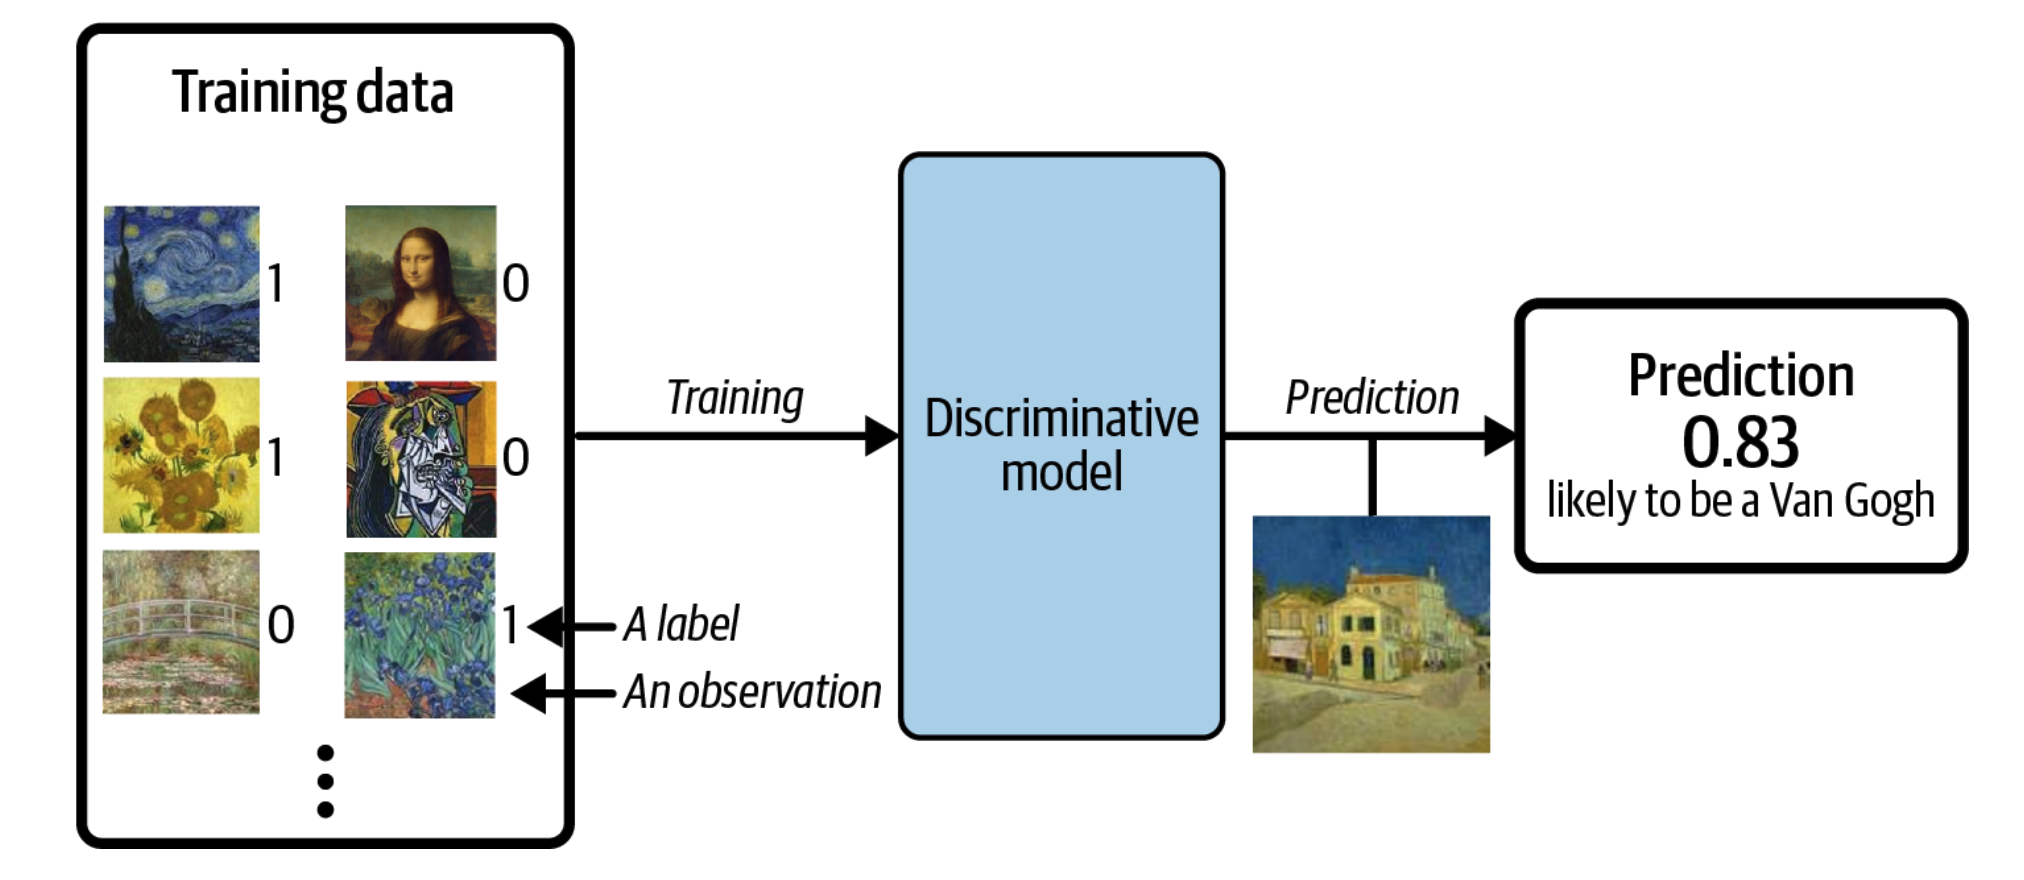
\includegraphics[width=1.0\linewidth]{figures/standarddeeplearning.png}}

\vspace{6mm}
\end{frame}

\begin{frame}[plain,fragile]
\frametitle{Example of generative modeling, \href{{https://www.oreilly.com/library/view/generative-deep-learning/9781098134174/ch01.html}}{taken from Generative Deep Learning by David Foster}}

\vspace{6mm}

% inline figure
\centerline{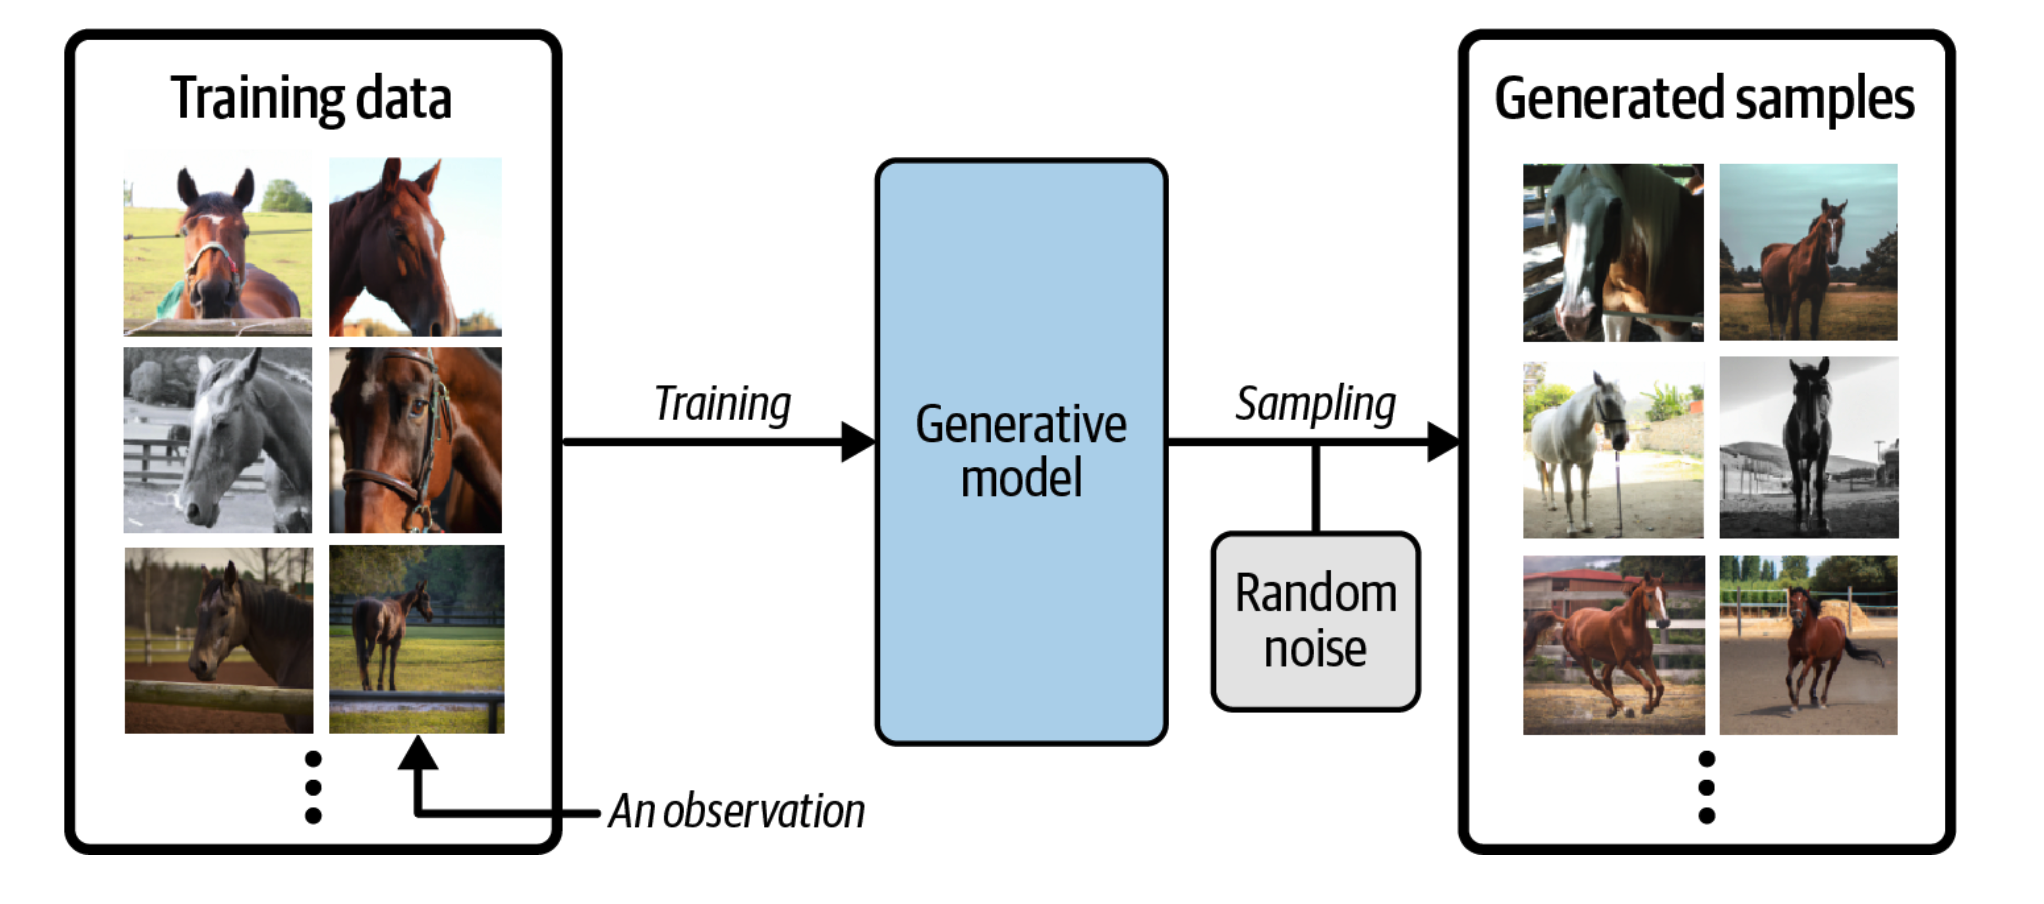
\includegraphics[width=1.0\linewidth]{figures/generativelearning.png}}

\vspace{6mm}
\end{frame}

\begin{frame}[plain,fragile]
\frametitle{Taxonomy of generative deep learning, \href{{https://www.oreilly.com/library/view/generative-deep-learning/9781098134174/ch01.html}}{taken from Generative Deep Learning by David Foster}}

\vspace{6mm}

% inline figure
\centerline{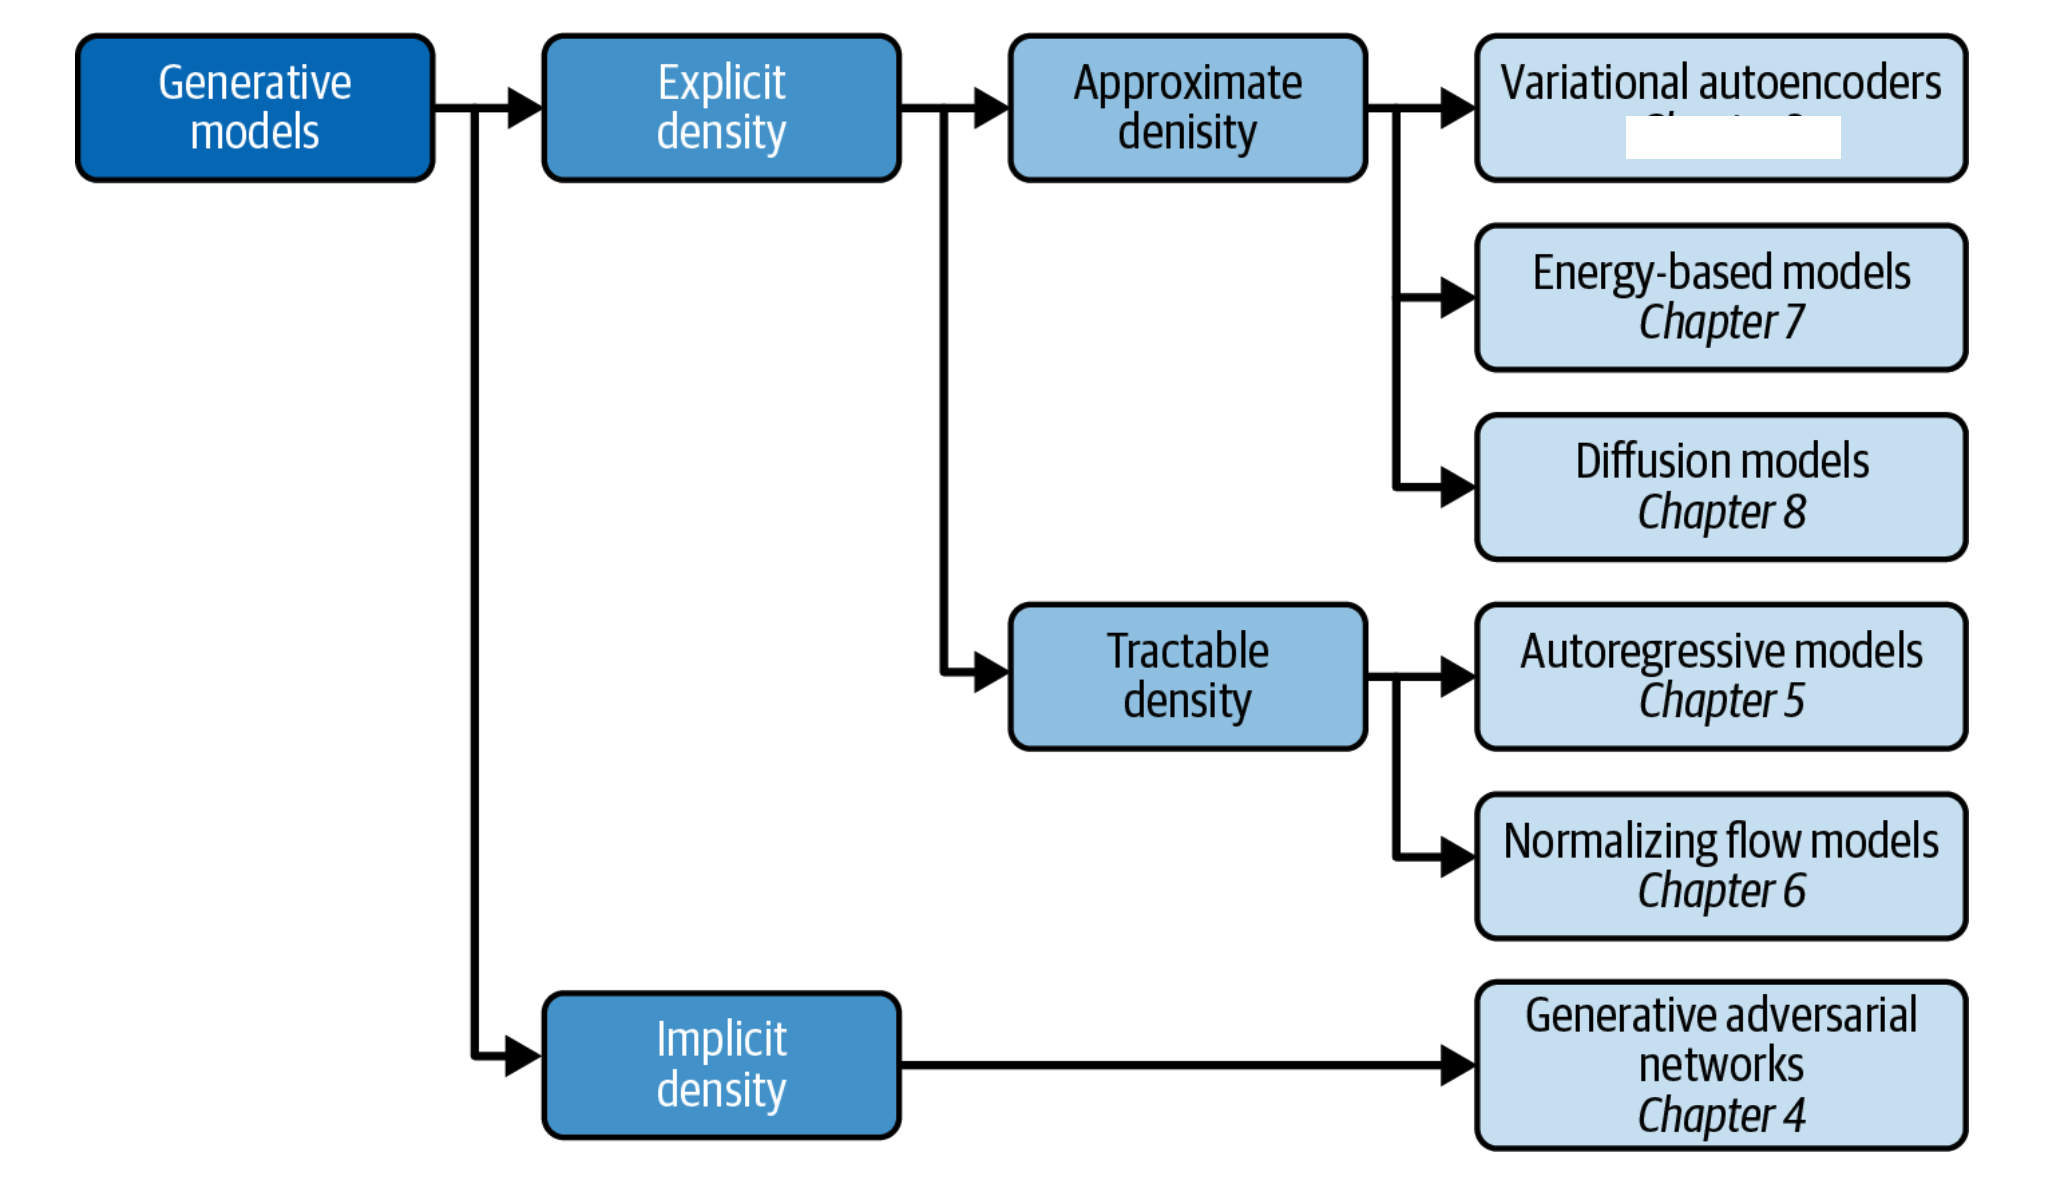
\includegraphics[width=1.0\linewidth]{figures/generativemodels.png}}

\vspace{6mm}
\end{frame}

\begin{frame}[plain,fragile]
\frametitle{Good books with hands-on material and codes}

\begin{block}{}
\begin{itemize}
\item \href{{https://sebastianraschka.com/blog/2022/ml-pytorch-book.html}}{Sebastian Rashcka et al, Machine learning with Sickit-Learn and PyTorch}

\item \href{{https://www.oreilly.com/library/view/generative-deep-learning/9781098134174/ch01.html}}{David Foster, Generative Deep Learning with TensorFlow}

\item \href{{https://github.com/PacktPublishing/Hands-On-Generative-AI-with-Python-and-TensorFlow-2}}{Babcock and Gavras, Generative AI with Python and TensorFlow 2}
\end{itemize}

\noindent
\end{block}

All three books have GitHub sites from where  one can download all codes. A good and more general text (2016)
is Goodfellow, Bengio and Courville, \href{{https://www.deeplearningbook.org/}}{Deep Learning}
\end{frame}

\begin{frame}[plain,fragile]
\frametitle{More references}

\begin{block}{Reading on diffusion models }
\begin{enumerate}
\item A central paper is the one by Sohl-Dickstein et al, Deep Unsupervised Learning using Nonequilibrium Thermodynamics, \href{{https://arxiv.org/abs/1503.03585}}{\nolinkurl{https://arxiv.org/abs/1503.03585}}

\item See also Diederik P. Kingma, Tim Salimans, Ben Poole, Jonathan Ho, Variational Diffusion Models, \href{{https://arxiv.org/abs/2107.00630}}{\nolinkurl{https://arxiv.org/abs/2107.00630}}
\end{enumerate}

\noindent
\end{block}   

\begin{block}{and VAEs }
\begin{enumerate}
\item An Introduction to Variational Autoencoders, by Kingma and Welling, see \href{{https://arxiv.org/abs/1906.02691}}{\nolinkurl{https://arxiv.org/abs/1906.02691}}
\end{enumerate}

\noindent
\end{block}

\textbf{And two Nobel prizes in 2024 (Chemistry and Physics!}
\end{frame}

\begin{frame}[plain,fragile]
\frametitle{What are the basic Machine Learning ingredients?}

\begin{block}{}
Almost every problem in ML and data science starts with the same ingredients:
\begin{itemize}
\item The dataset $\bm{x}$ (could be some observable quantity of the system we are studying)

\item A model which is a function of a set of parameters $\bm{\alpha}$ that relates to the dataset, say a likelihood  function $p(\bm{x}\vert \bm{\alpha})$ or just a simple model $f(\bm{\alpha})$

\item A so-called \textbf{loss/cost/risk} function $\mathcal{C} (\bm{x}, f(\bm{\alpha}))$ which allows us to decide how well our model represents the dataset. 
\end{itemize}

\noindent
We seek to minimize the function $\mathcal{C} (\bm{x}, f(\bm{\alpha}))$ by finding the parameter values which minimize $\mathcal{C}$. This leads to  various minimization algorithms. It may surprise many, but at the heart of all machine learning algortihms there is an optimization problem. 
\end{block}
\end{frame}

\begin{frame}[plain,fragile]
\frametitle{Low-level machine learning, the family of ordinary least squares methods}

Our data which we want to apply a machine learning method on, consist
of a set of inputs $\bm{x}^T=[x_0,x_1,x_2,\dots,x_{n-1}]$ and the
outputs we want to model $\bm{y}^T=[y_0,y_1,y_2,\dots,y_{n-1}]$.
We assume  that the output data can be represented (for a regression case) by a continuous function $f$
through
\[
\bm{y}=f(\bm{x})+\bm{\epsilon}.
\]
\end{frame}

\begin{frame}[plain,fragile]
\frametitle{Setting up the equations}

In linear regression we approximate the unknown function with another
continuous function $\tilde{\bm{y}}(\bm{x})$ which depends linearly on
some unknown parameters
$\bm{\theta}^T=[\theta_0,\theta_1,\theta_2,\dots,\theta_{p-1}]$.

The input data can be organized in terms of a so-called design matrix 
with an approximating function $\bm{\tilde{y}}$ 
\[
\bm{\tilde{y}}= \bm{X}\bm{\theta},
\]
\end{frame}

\begin{frame}[plain,fragile]
\frametitle{The objective/cost/loss function}

The  simplest approach is the mean squared error
\[
C(\bm{\Theta})=\frac{1}{n}\sum_{i=0}^{n-1}\left(y_i-\tilde{y}_i\right)^2=\frac{1}{n}\left\{\left(\bm{y}-\bm{\tilde{y}}\right)^T\left(\bm{y}-\bm{\tilde{y}}\right)\right\},
\]
or using the matrix $\bm{X}$ and in a more compact matrix-vector notation as
\[
C(\bm{\Theta})=\frac{1}{n}\left\{\left(\bm{y}-\bm{X}\bm{\theta}\right)^T\left(\bm{y}-\bm{X}\bm{\theta}\right)\right\}.
\]
This function represents one of many possible ways to define the so-called cost function.
\end{frame}

\begin{frame}[plain,fragile]
\frametitle{Training solution}

Optimizing with respect to the unknown parameters $\theta_j$ we get 
\[
\bm{X}^T\bm{y} = \bm{X}^T\bm{X}\bm{\theta},  
\]
and if the matrix $\bm{X}^T\bm{X}$ is invertible we have the optimal values
\[
\hat{\bm{\theta}} =\left(\bm{X}^T\bm{X}\right)^{-1}\bm{X}^T\bm{y}.
\]

We say we 'learn' the unknown parameters $\bm{\theta}$ from the last equation.
\end{frame}

\begin{frame}[plain,fragile]
\frametitle{Selected references}

\begin{block}{}
\begin{itemize}
\item \href{{https://arxiv.org/abs/1803.08823}}{Mehta et al.} and \href{{https://www.sciencedirect.com/science/article/pii/S0370157319300766?via%3Dihub}}{Physics Reports (2019)}.

\item \href{{https://link.aps.org/doi/10.1103/RevModPhys.91.045002}}{Machine Learning and the Physical Sciences by Carleo et al}

\item \href{{https://journals.aps.org/rmp/abstract/10.1103/RevModPhys.94.031003}}{Artificial Intelligence and Machine Learning in Nuclear Physics, Amber Boehnlein et al., Reviews Modern of Physics 94, 031003 (2022)} 

\item \href{{https://journals.aps.org/prresearch/pdf/10.1103/PhysRevResearch.5.033062}}{Dilute neutron star matter from neural-network quantum states by Fore et al, Physical Review Research 5, 033062 (2023)}

\item Neural-network quantum states for ultra-cold Fermi gases, Jane Kim et al, Commun Phys 7, 148 (2024), see \href{{https://doi.org/10.48550/arXiv.2305.08831}}{\nolinkurl{https://doi.org/10.48550/arXiv.2305.08831}}
\end{itemize}

\noindent
\end{block}
\end{frame}

\begin{frame}[plain,fragile]
\frametitle{Scientific Machine Learning}

An important and emerging field is what has been dubbed as scientific ML, see the article by Deiana et al "Applications and Techniques for Fast Machine Learning in Science, Big Data \textbf{5}, 787421 (2022):https://doi.org/10.3389/fdata.2022.787421"

\begin{block}{}
The authors discuss applications and techniques for fast machine
learning (ML) in science -- the concept of integrating power ML
methods into the real-time experimental data processing loop to
accelerate scientific discovery. The report covers three main areas

\begin{enumerate}
\item applications for fast ML across a number of scientific domains;

\item techniques for training and implementing performant and resource-efficient ML algorithms;

\item and computing architectures, platforms, and technologies for deploying these algorithms.
\end{enumerate}

\noindent
\end{block}
\end{frame}

\begin{frame}[plain,fragile]
\frametitle{And more}

\begin{block}{}
\begin{itemize}
\item An important application of AI/ML methods is to improve the estimation of bias or uncertainty due to the introduction of or lack of physical constraints in various theoretical models.

\item In theory, we expect to use AI/ML algorithms and methods to improve our knowledge about  correlations of physical model parameters in data for quantum many-body systems. Deep learning methods show great promise in circumventing the exploding dimensionalities encountered in quantum mechanical many-body studies. 

\item Merging a frequentist approach (the standard path in ML theory) with a Bayesian approach, has the potential to infer better probabilitity distributions and error estimates. 

\item Machine Learning and Quantum Computing is a very interesting avenue
\end{itemize}

\noindent
\end{block}
\end{frame}

\begin{frame}[plain,fragile]
\frametitle{Many-body physics, Quantum Monte Carlo and deep learning}

\begin{block}{}
Given a hamiltonian $H$ and a trial wave function $\Psi_T$, the variational principle states that the expectation value of $\langle H \rangle$, defined through 
\[
   \langle E \rangle =
   \frac{\int d\bm{R}\Psi^{\ast}_T(\bm{R})H(\bm{R})\Psi_T(\bm{R})}
        {\int d\bm{R}\Psi^{\ast}_T(\bm{R})\Psi_T(\bm{R})},
\]
is an upper bound to the ground state energy $E_0$ of the hamiltonian $H$, that is 
\[
    E_0 \le \langle E \rangle.
\]
In general, the integrals involved in the calculation of various  expectation values  are multi-dimensional ones. Traditional integration methods such as the Gauss-Legendre will not be adequate for say the  computation of the energy of a many-body system.  \textbf{Basic philosophy: Let a neural network find the optimal wave function}
\end{block}
\end{frame}

\begin{frame}[plain,fragile]
\frametitle{Quantum Monte Carlo Motivation}

\begin{block}{Basic steps }
Choose a trial wave function
$\psi_T(\bm{R})$.
\[
   P(\bm{R},\bm{\alpha})= \frac{\left|\psi_T(\bm{R},\bm{\alpha})\right|^2}{\int \left|\psi_T(\bm{R},\bm{\alpha})\right|^2d\bm{R}}.
\]
This is our model, or likelihood/probability distribution function  (PDF). It depends on some variational parameters $\bm{\alpha}$.
The approximation to the expectation value of the Hamiltonian is now 
\[
   \langle E[\bm{\alpha}] \rangle = 
   \frac{\int d\bm{R}\Psi^{\ast}_T(\bm{R},\bm{\alpha})H(\bm{R})\Psi_T(\bm{R},\bm{\alpha})}
        {\int d\bm{R}\Psi^{\ast}_T(\bm{R},\bm{\alpha})\Psi_T(\bm{R},\bm{\alpha})}.
\]
\end{block}
\end{frame}

\begin{frame}[plain,fragile]
\frametitle{Quantum Monte Carlo Motivation}

\begin{block}{Define a new quantity }
\[
   E_L(\bm{R},\bm{\alpha})=\frac{1}{\psi_T(\bm{R},\bm{\alpha})}H\psi_T(\bm{R},\bm{\alpha}),
\]
called the local energy, which, together with our trial PDF yields
\[
  \langle E[\bm{\alpha}] \rangle=\int P(\bm{R})E_L(\bm{R},\bm{\alpha}) d\bm{R}\approx \frac{1}{N}\sum_{i=1}^NE_L(\bm{R_i},\bm{\alpha})
\]
with $N$ being the number of Monte Carlo samples.
\end{block}
\end{frame}

\begin{frame}[plain,fragile]
\frametitle{Energy derivatives}

\begin{block}{}
The local energy as function of the variational parameters defines now our \textbf{objective/cost} function.

To find the derivatives of the local energy expectation value as function of the variational parameters, we can use the chain rule and the hermiticity of the Hamiltonian.  

Let us define (with the notation $\langle E[\bm{\alpha}]\rangle =\langle  E_L\rangle$)
\[
\bar{E}_{\alpha_i}=\frac{d\langle  E_L\rangle}{d\alpha_i},
\]
as the derivative of the energy with respect to the variational parameter $\alpha_i$
We define also the derivative of the trial function (skipping the subindex $T$) as 
\[
\bar{\Psi}_{i}=\frac{d\Psi}{d\alpha_i}.
\]
\end{block}
\end{frame}

\begin{frame}[plain,fragile]
\frametitle{Derivatives of the local energy}

\begin{block}{}
The elements of the gradient of the local energy are 
\[
\bar{E}_{i}= 2\left( \langle \frac{\bar{\Psi}_{i}}{\Psi}E_L\rangle -\langle \frac{\bar{\Psi}_{i}}{\Psi}\rangle\langle E_L \rangle\right).
\]
From a computational point of view it means that you need to compute the expectation values of 
\[
\langle \frac{\bar{\Psi}_{i}}{\Psi}E_L\rangle,
\]
and
\[
\langle \frac{\bar{\Psi}_{i}}{\Psi}\rangle\langle E_L\rangle
\]
These integrals are evaluted using MC intergration (with all its possible error sources). Use methods like stochastic gradient or other minimization methods to find the optimal parameters.
\end{block}
\end{frame}

\begin{frame}[plain,fragile]
\frametitle{Why Feed Forward Neural Networks (FFNN)?}

\begin{block}{}
According to the \emph{Universal approximation theorem}, a feed-forward
neural network with just a single hidden layer containing a finite
number of neurons can approximate a continuous multidimensional
function to arbitrary accuracy.
\end{block}
\end{frame}

\begin{frame}[plain,fragile]
\frametitle{Universal approximation theorem}

The universal approximation theorem plays a central role in deep
learning.  \href{{https://link.springer.com/article/10.1007/BF02551274}}{Cybenko (1989)} showed
the following:

\begin{block}{}
Let $\sigma$ be any continuous sigmoidal function such that
\[
\sigma(z) = \left\{\begin{array}{cc} 1 & z\rightarrow \infty\\ 0 & z \rightarrow -\infty \end{array}\right.
\]
Given a continuous and deterministic function $F(\bm{x})$ on the unit
cube in $d$-dimensions $F\in [0,1]^d$, $x\in [0,1]^d$ and a parameter
$\epsilon >0$, there is a one-layer (hidden) neural network
$f(\bm{x};\bm{\Theta})$ with $\bm{\Theta}=(\bm{W},\bm{b})$ and $\bm{W}\in
\mathbb{R}^{m\times n}$ and $\bm{b}\in \mathbb{R}^{n}$, for which
\[
\vert F(\bm{x})-f(\bm{x};\bm{\Theta})\vert < \epsilon \hspace{0.1cm} \forall \bm{x}\in[0,1]^d.
\]

\end{block}
\end{frame}

\begin{frame}[plain,fragile]
\frametitle{The approximation theorem in words}

\textbf{Any continuous function $y=F(\bm{x})$ supported on the unit cube in
$d$-dimensions can be approximated by a one-layer sigmoidal network to
arbitrary accuracy.}

\href{{https://www.sciencedirect.com/science/article/abs/pii/089360809190009T}}{Hornik (1991)} extended the theorem by letting any non-constant, bounded activation function to be included using that the expectation value
\[
\mathbb{E}[\vert F(\bm{x})\vert^2] =\int_{\bm{x}\in D} \vert F(\bm{x})\vert^2p(\bm{x})d\bm{x} < \infty.
\]
Then we have
\[
\mathbb{E}[\vert F(\bm{x})-f(\bm{x};\bm{\Theta})\vert^2] =\int_{\bm{x}\in D} \vert F(\bm{x})-f(\bm{x};\bm{\Theta})\vert^2p(\bm{x})d\bm{x} < \epsilon.
\]
\end{frame}

\begin{frame}[plain,fragile]
\frametitle{More on the general approximation theorem}

None of the proofs give any insight into the relation between the
number of of hidden layers and nodes and the approximation error
$\epsilon$, nor the magnitudes of $\bm{W}$ and $\bm{b}$.

Neural networks (NNs) have what we may call a kind of universality no matter what function we want to compute.

\begin{block}{}
It does not mean that an NN can be used to exactly compute any function. Rather, we get an approximation that is as good as we want. 
\end{block}
\end{frame}

\begin{frame}[plain,fragile]
\frametitle{Class of functions we can approximate}

\begin{block}{}
The class of functions that can be approximated are the continuous ones.
If the function $F(\bm{x})$ is discontinuous, it won't in general be possible to approximate it. However, an NN may still give an approximation even if we fail in some points.
\end{block}
\end{frame}

\begin{frame}[plain,fragile]
\frametitle{Monte Carlo methods and Neural Networks}

\href{{https://www.sciencedirect.com/science/article/pii/S0370269320305463?via%3Dihub}}{Machine Learning and the Deuteron by Kebble and Rios} and
\href{{https://journals.aps.org/prl/abstract/10.1103/PhysRevLett.127.022502}}{Variational Monte Carlo calculations of $A\le 4$ nuclei with an artificial neural-network correlator ansatz by Adams et al.}

\textbf{Adams et al}:

\begin{align}
H_{LO} &=-\sum_i \frac{{\vec{\nabla}_i^2}}{2m_N}
+\sum_{i<j} {\left(C_1  + C_2\, \vec{\sigma_i}\cdot\vec{\sigma_j}\right)
e^{-r_{ij}^2\Lambda^2 / 4 }}
\nonumber\\
&+D_0 \sum_{i<j<k} \sum_{\text{cyc}}
{e^{-\left(r_{ik}^2+r_{ij}^2\right)\Lambda^2/4}}\,,
\end{align}

where $m_N$ is the mass of the nucleon, $\vec{\sigma_i}$ is the Pauli
matrix acting on nucleon $i$, and $\sum_{\text{cyc}}$ stands for the
cyclic permutation of $i$, $j$, and $k$. The low-energy constants
$C_1$ and $C_2$ are fit to the deuteron binding energy and to the
neutron-neutron scattering length
\end{frame}

\begin{frame}[plain,fragile]
\frametitle{Deep learning neural networks, \href{{https://journals.aps.org/prl/abstract/10.1103/PhysRevLett.127.022502}}{Variational Monte Carlo calculations of $A\le 4$ nuclei with an artificial neural-network correlator ansatz by Adams et al.}}

An appealing feature of the neural network ansatz is that it is more general than the more conventional product of two-
and three-body spin-independent Jastrow functions
\begin{align}
|\Psi_V^J \rangle = \prod_{i<j<k} \Big( 1-\sum_{\text{cyc}} u(r_{ij}) u(r_{jk})\Big) \prod_{i<j} f(r_{ij}) | \Phi\rangle\,,
\end{align}
which is commonly used for nuclear Hamiltonians that do not contain tensor and spin-orbit terms.
The above function is typically replaced by a  deep Neural Network.
\end{frame}

\begin{frame}[plain,fragile]
\frametitle{Ansatz for a fermionic state function, Jane Kim et al, Commun Phys 7, 148 (2024)}

\[
\Psi_T(\bm{X}) =\exp{U(\bm{X})}\Phi(\bm{X}).
\]

\begin{block}{}
\begin{enumerate}
\item Build in fermion antisymmetry for network compactness

\item Permutation-invariant Jastrow function improves ansatz flexibility

\item Build $U$ and $\Phi$ functions from fully connected, deep neural networks

\item Use Slater determinant (or Pfaffian) $\Phi$ to enforce antisymmetry with single particle wavefunctions represented by neural networks
\end{enumerate}

\noindent
\end{block}
\end{frame}

\begin{frame}[plain,fragile]
\frametitle{Nuclear matter setup}

\vspace{6mm}

% inline figure
\centerline{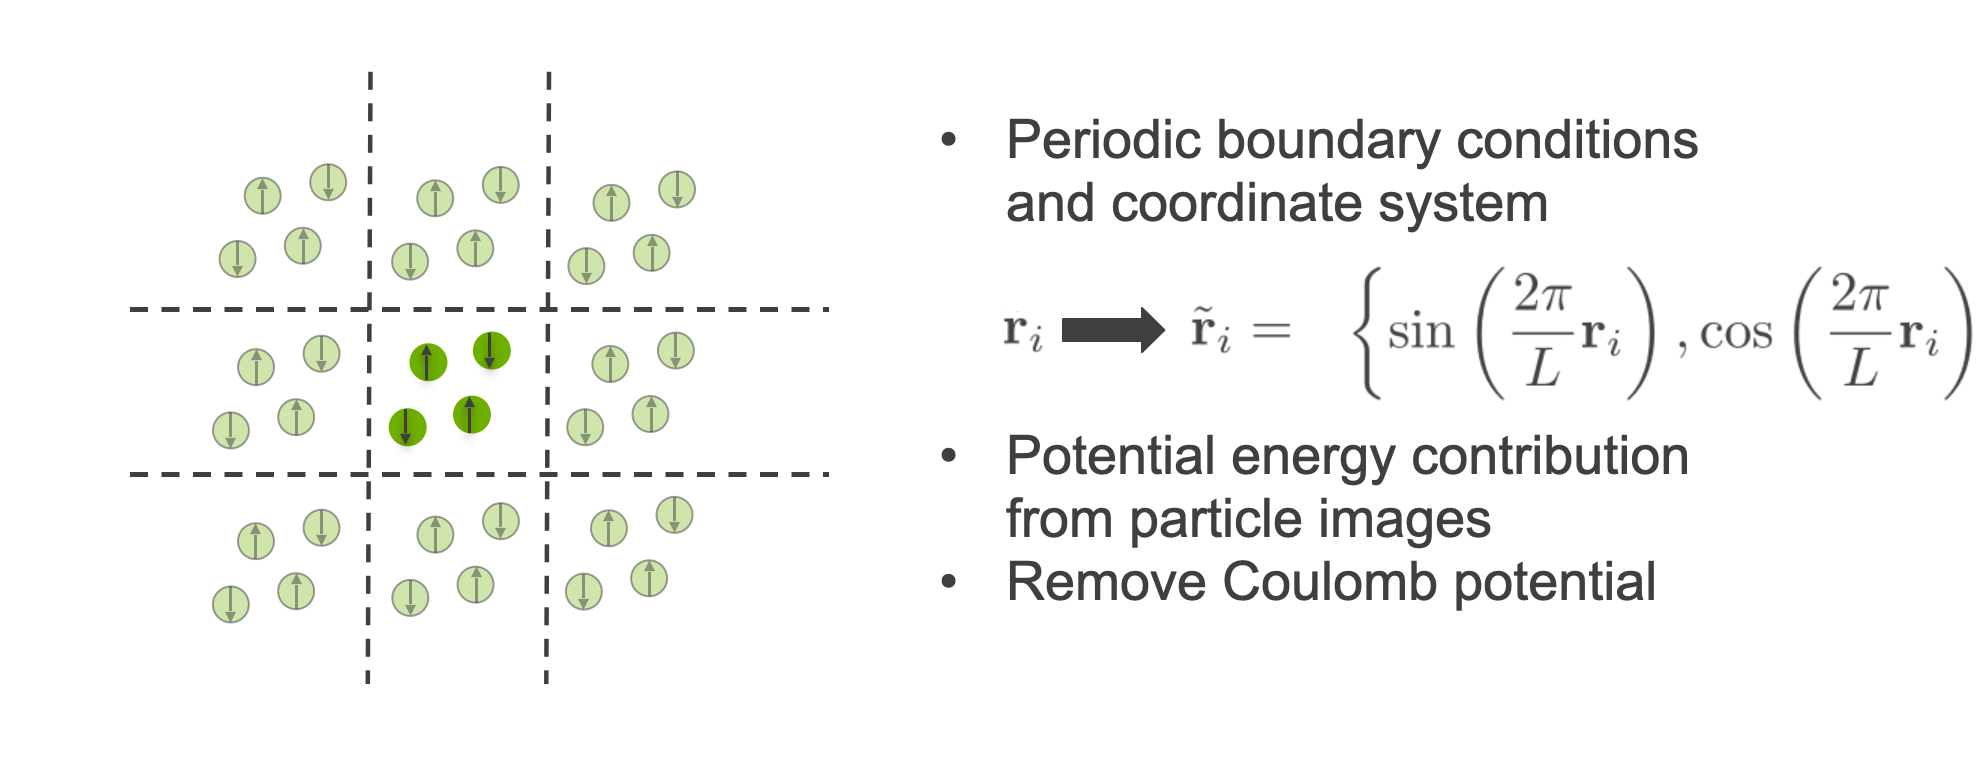
\includegraphics[width=1.0\linewidth]{figures/mbpfig4.png}}

\vspace{6mm}
\end{frame}

\begin{frame}[plain,fragile]
\frametitle{Neutron star structure}

\vspace{6mm}

% inline figure
\centerline{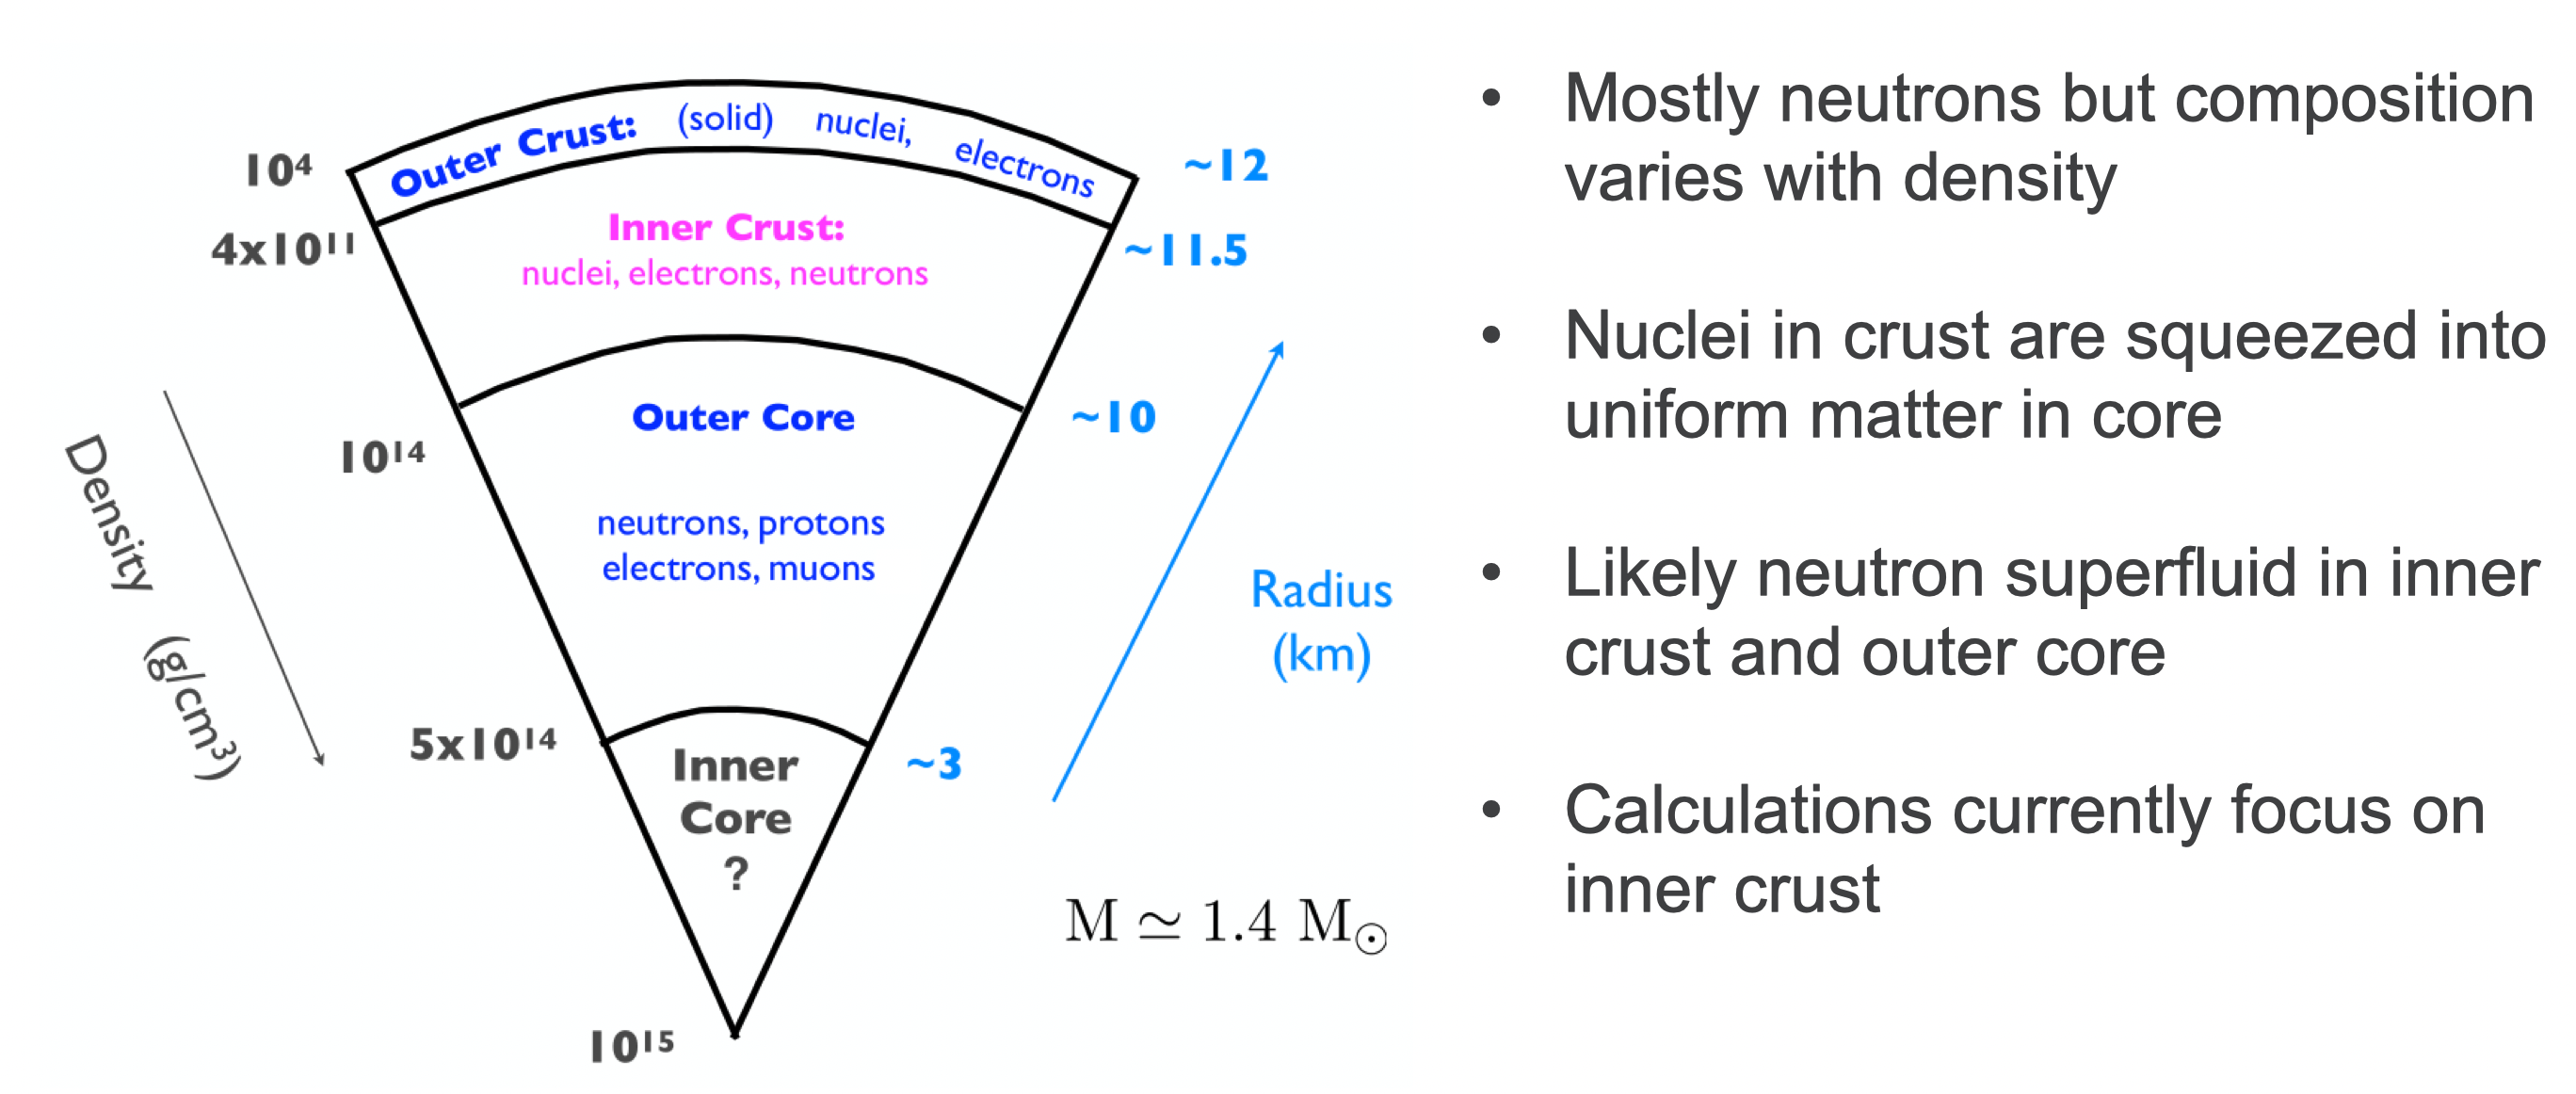
\includegraphics[width=1.0\linewidth]{figures/mbpfig5.png}}

\vspace{6mm}
\end{frame}

\begin{frame}[plain,fragile]
\frametitle{\href{{https://journals.aps.org/prresearch/pdf/10.1103/PhysRevResearch.5.033062}}{Dilute neutron star matter from neural-network quantum states by Fore et al, Physical Review Research 5, 033062 (2023)} at density $\rho=0.04$ fm$^{-3}$}

\begin{block}{}

\vspace{6mm}

% inline figure
\centerline{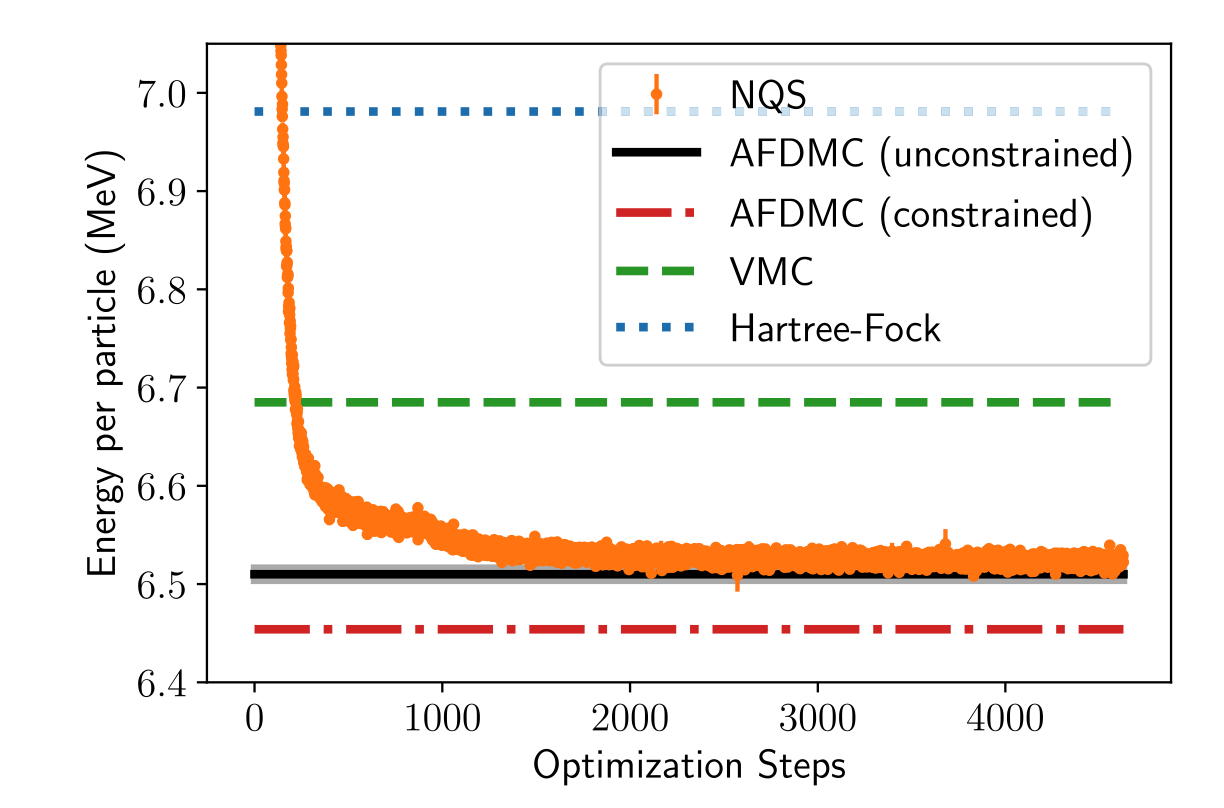
\includegraphics[width=0.9\linewidth]{figures/nmatter.png}}

\vspace{6mm}

\end{block}
\end{frame}

\begin{frame}[plain,fragile]
\frametitle{Pairing and Spin-singlet and triplet two-body distribution functions at $\rho=0.01$ fm$^{-3}$}

\begin{block}{}

\vspace{6mm}

% inline figure
\centerline{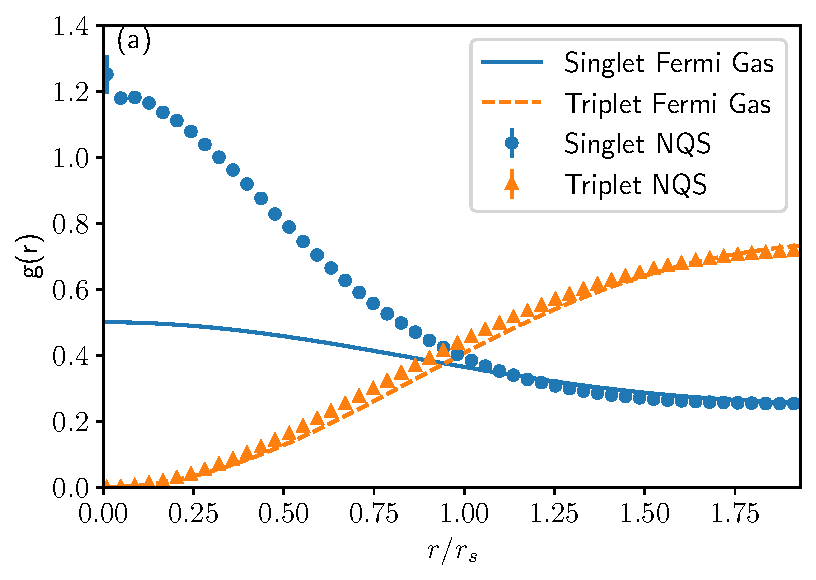
\includegraphics[width=0.9\linewidth]{figures/01_tbd.pdf}}

\vspace{6mm}

\end{block}
\end{frame}

\begin{frame}[plain,fragile]
\frametitle{Pairing and Spin-singlet and triplet two-body distribution functions at $\rho=0.04$ fm$^{-3}$}

\begin{block}{}

\vspace{6mm}

% inline figure
\centerline{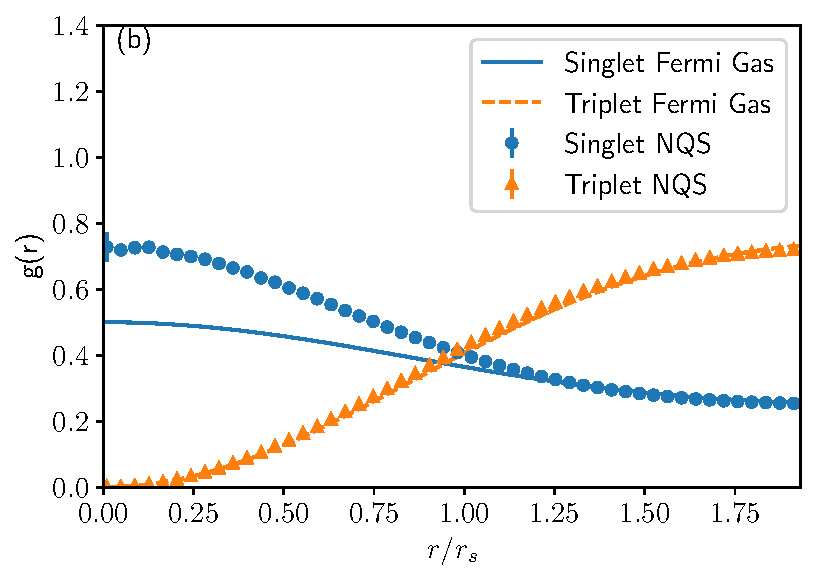
\includegraphics[width=0.9\linewidth]{figures/04_tbd.pdf}}

\vspace{6mm}

\end{block}
\end{frame}

\begin{frame}[plain,fragile]
\frametitle{Pairing and Spin-singlet and triplet two-body distribution functions at $\rho=0.08$ fm$^{-3}$}

\begin{block}{}

\vspace{6mm}

% inline figure
\centerline{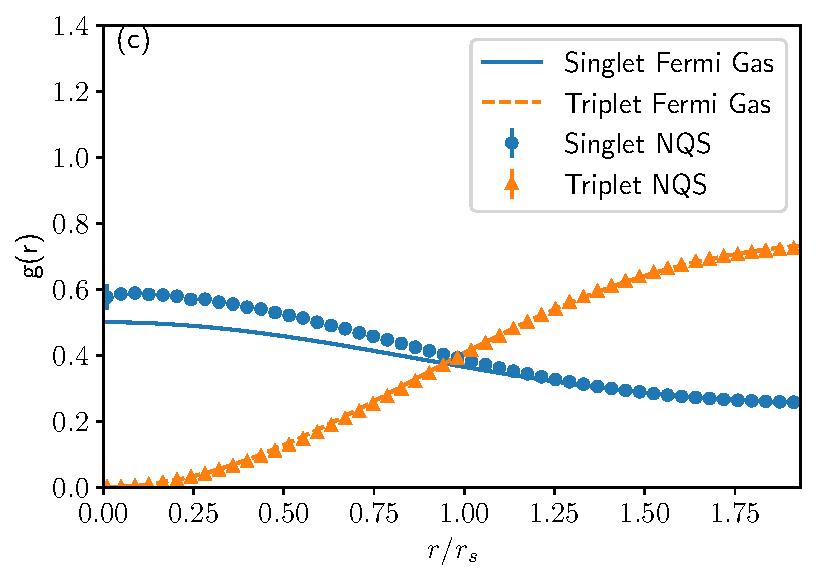
\includegraphics[width=0.9\linewidth]{figures/08_tbd.pdf}}

\vspace{6mm}

\end{block}
\end{frame}

\begin{frame}[plain,fragile]
\frametitle{Self-emerging clustering}

\vspace{6mm}

% inline figure
\centerline{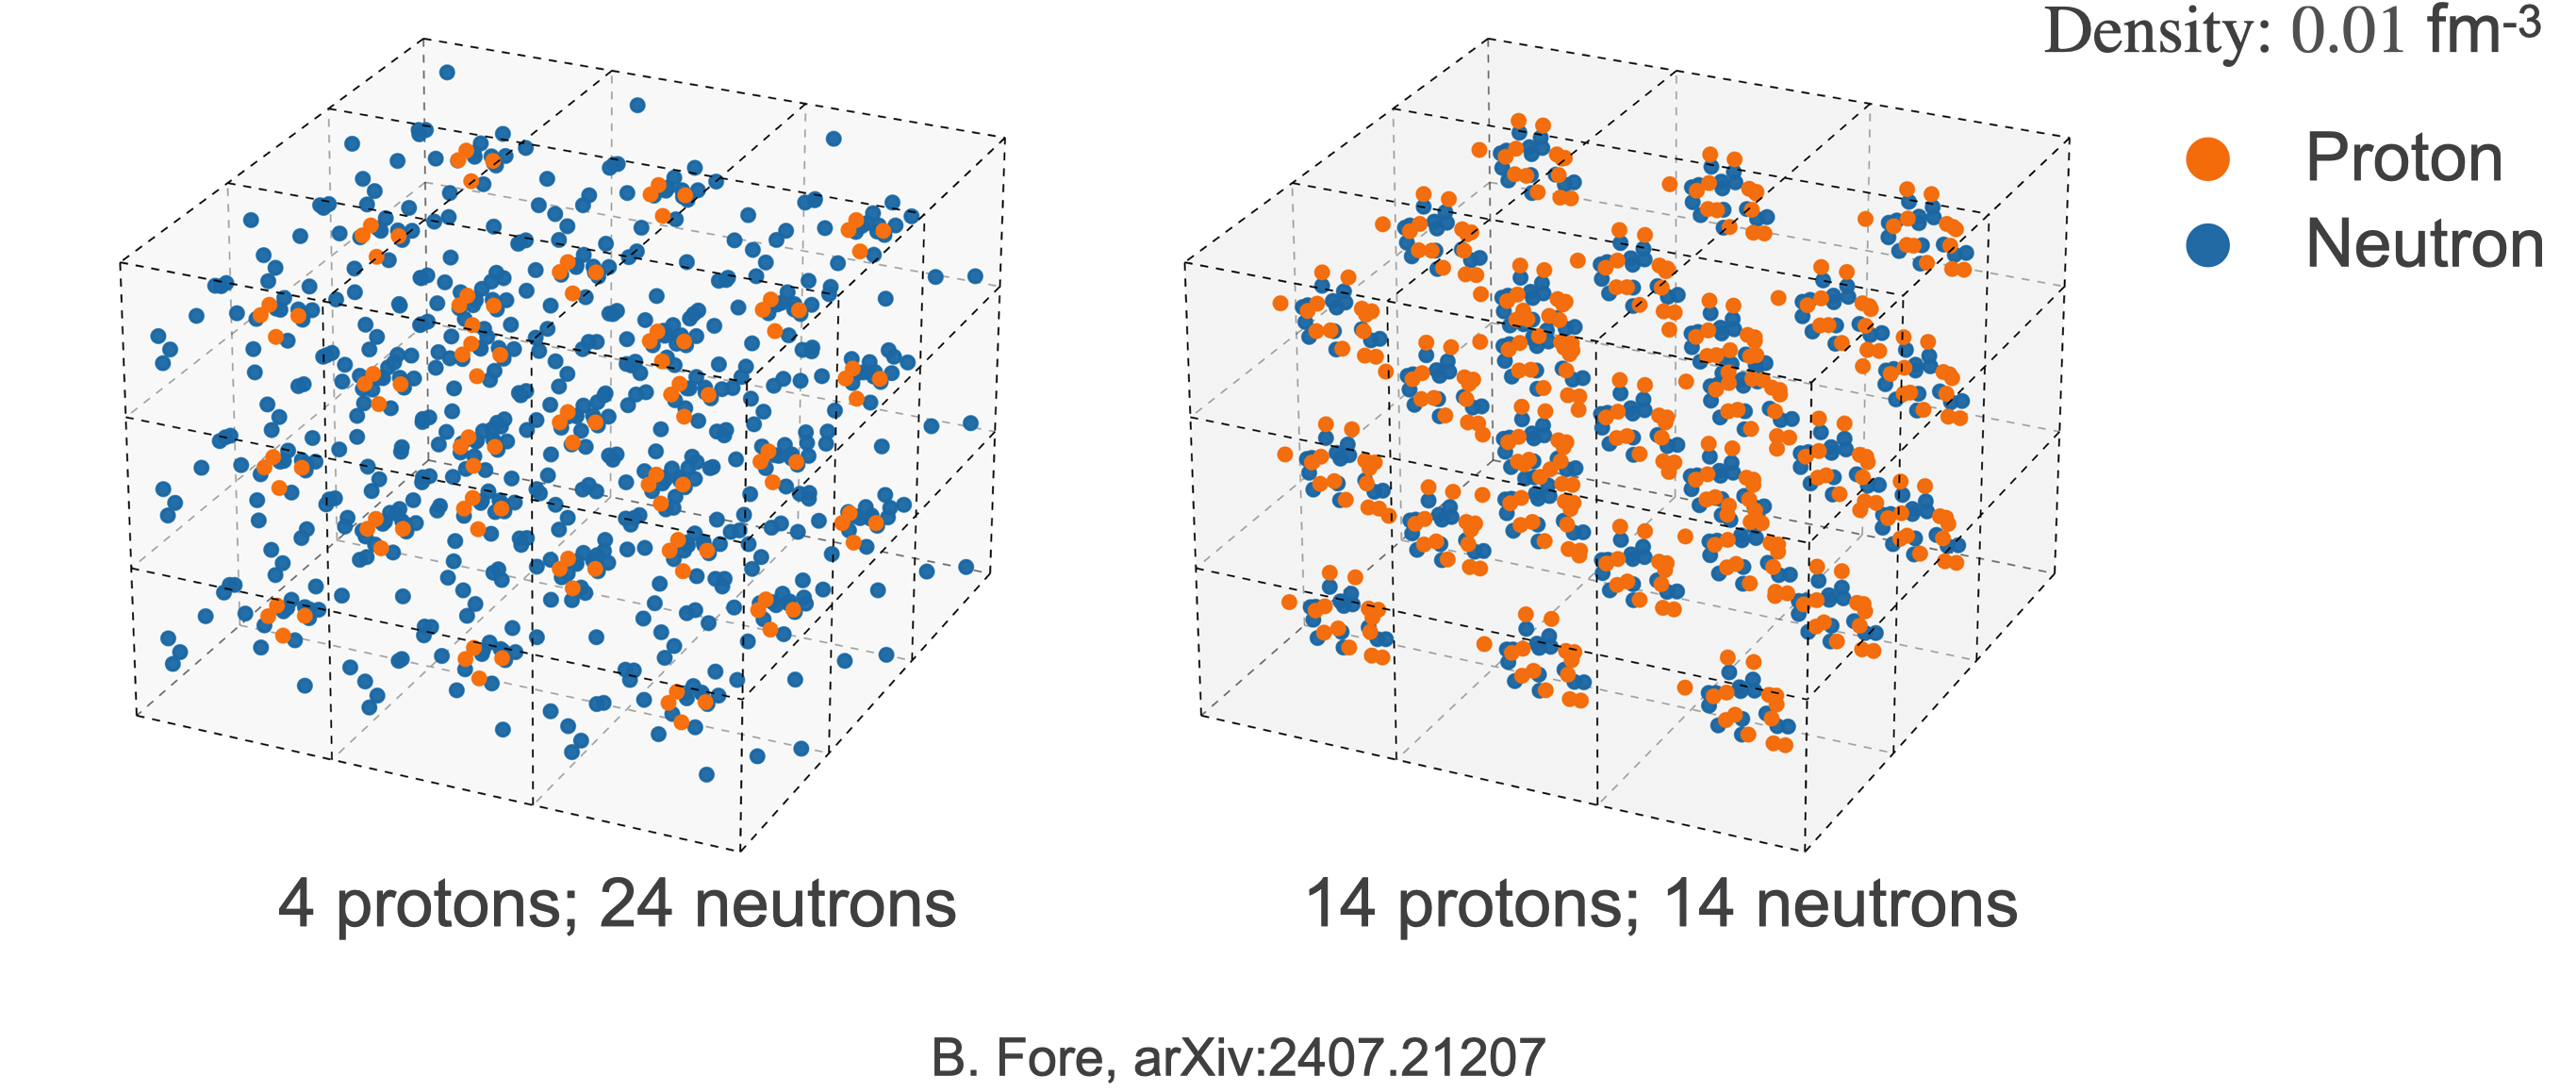
\includegraphics[width=1.0\linewidth]{figures/mbpfig7.png}}

\vspace{6mm}
\end{frame}

\begin{frame}[plain,fragile]
\frametitle{Clustering: Two-body pair distributions}

\vspace{6mm}

% inline figure
\centerline{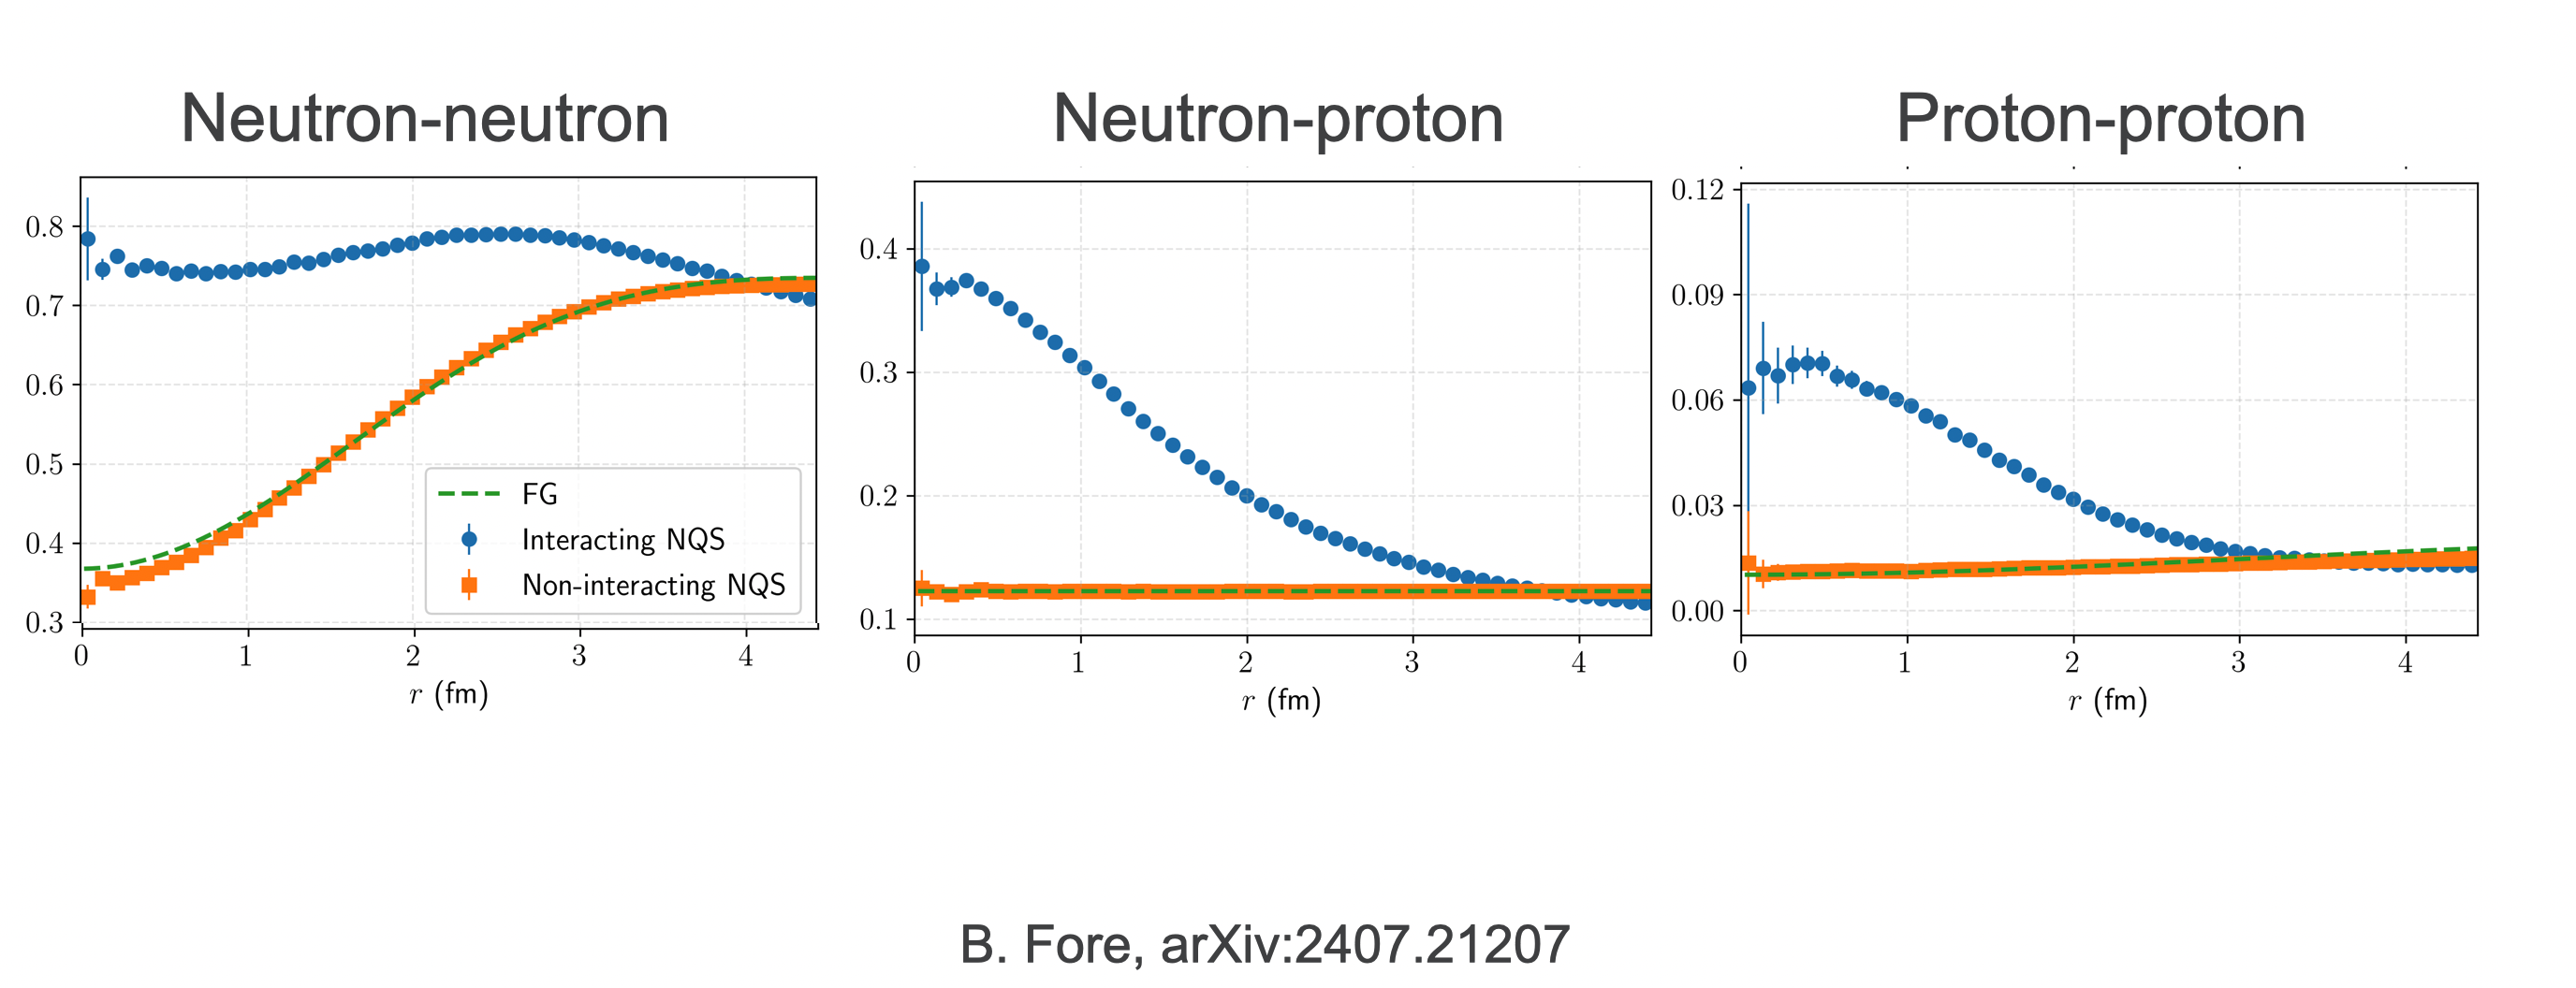
\includegraphics[width=1.0\linewidth]{figures/mbpfig8.png}}

\vspace{6mm}
\end{frame}

\begin{frame}[plain,fragile]
\frametitle{Nuclear matter proton fraction}

\vspace{6mm}

% inline figure
\centerline{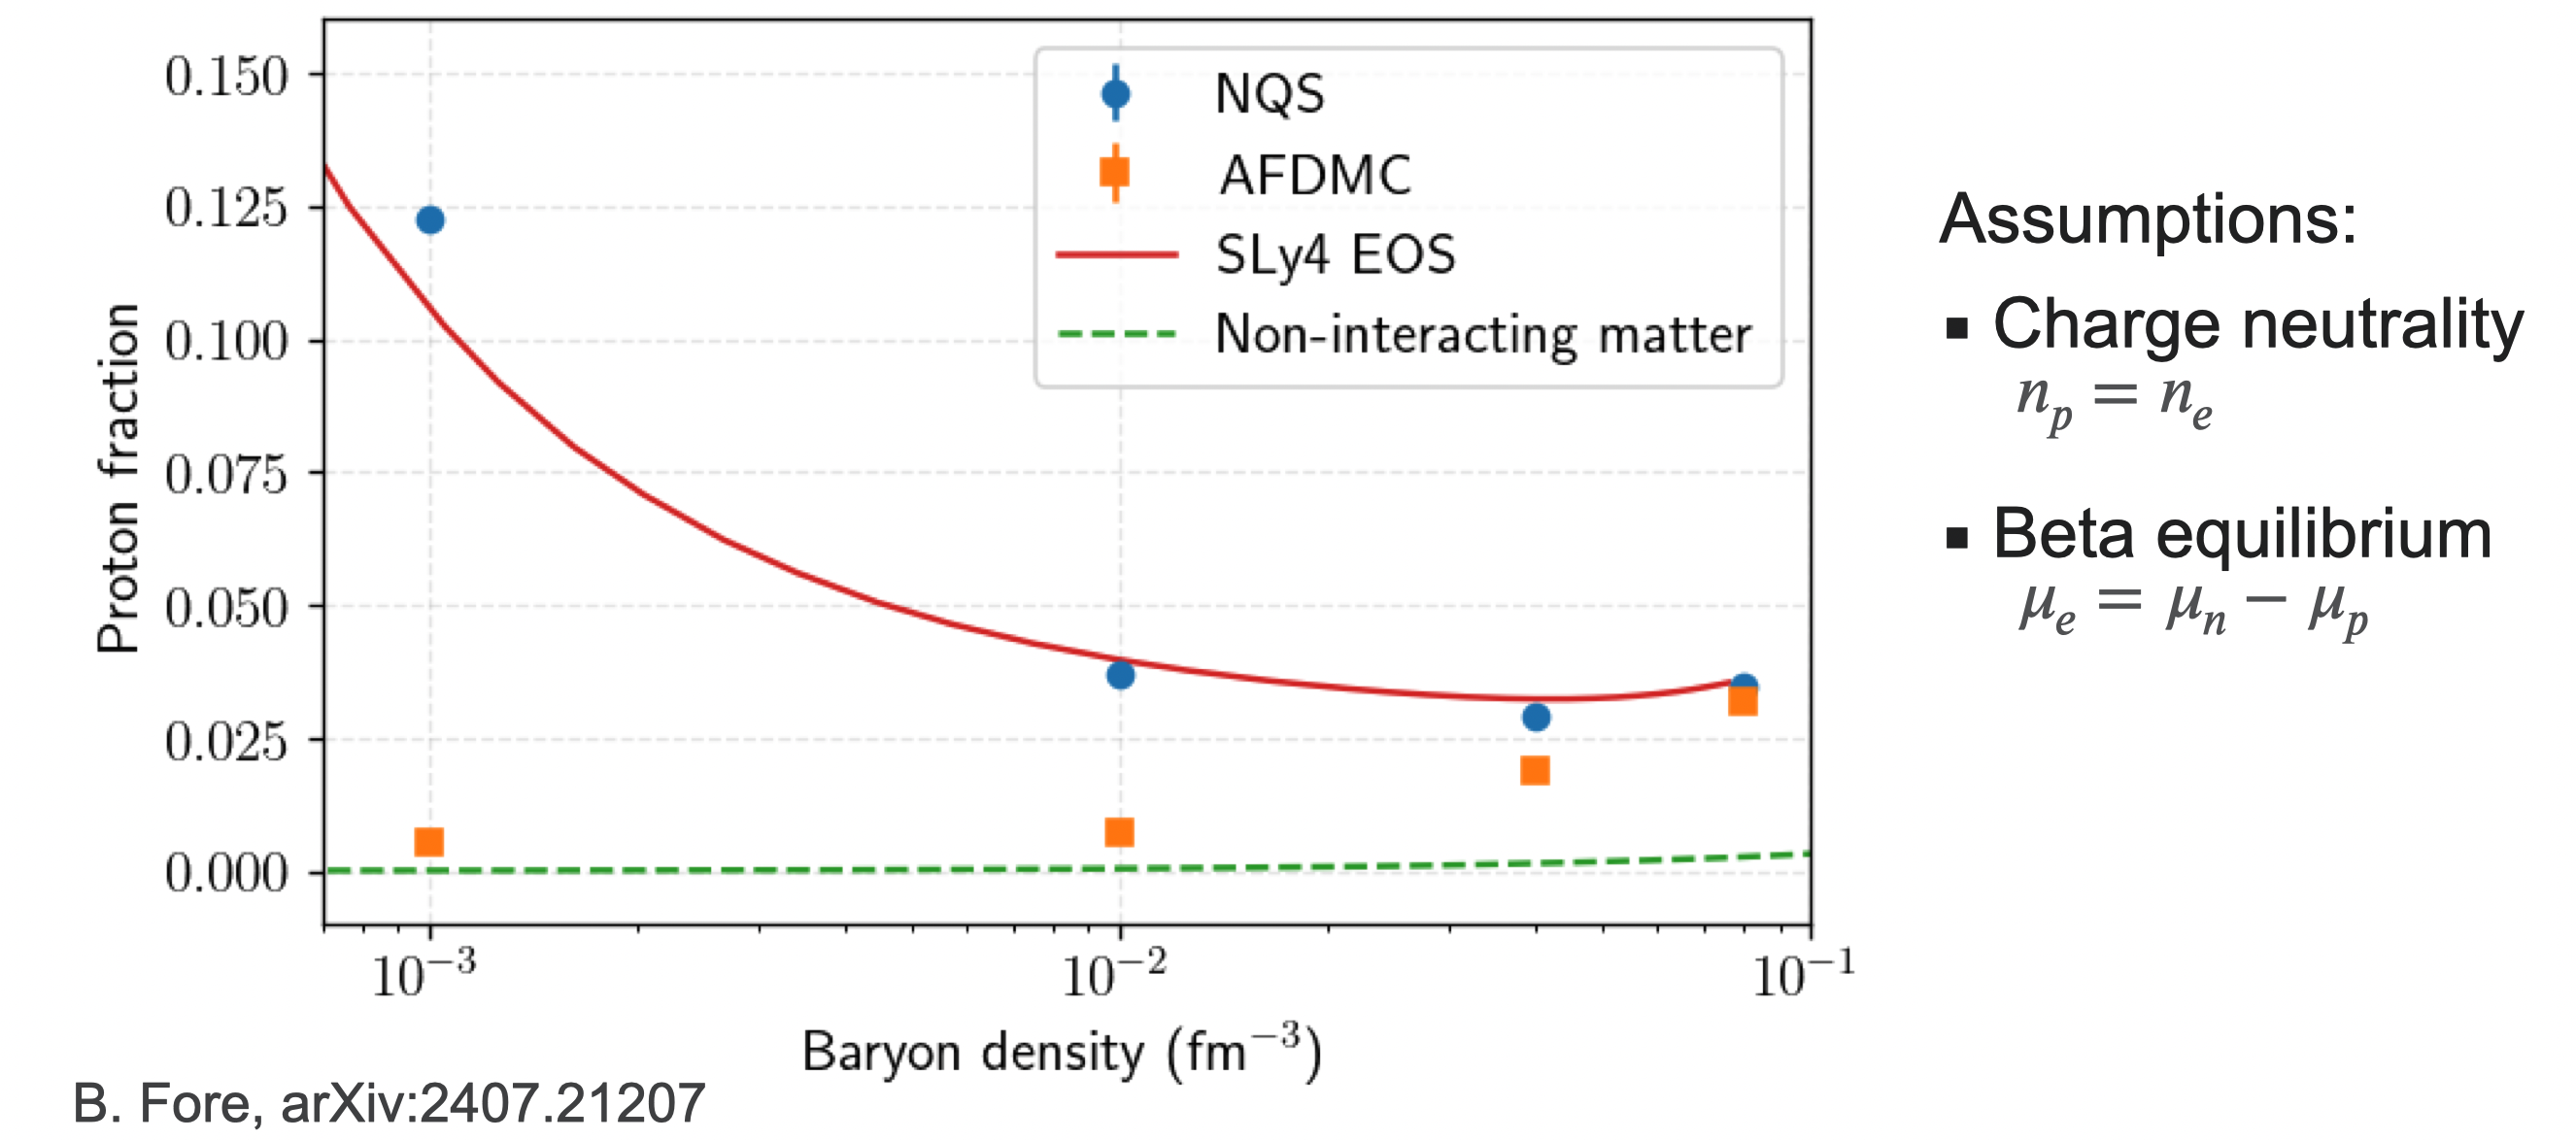
\includegraphics[width=1.0\linewidth]{figures/mbpfig9.png}}

\vspace{6mm}
\end{frame}

\begin{frame}[plain,fragile]
\frametitle{The electron gas in three dimensions with $N=14$ electrons (Wigner-Seitz radius $r_s=2$ a.u.), \href{{https://journals.aps.org/prb/abstract/10.1103/PhysRevB.110.035108}}{Gabriel Pescia, Jane Kim et al.~PRB 110, 035108 (2024),}}

\begin{block}{}

\vspace{6mm}

% inline figure
\centerline{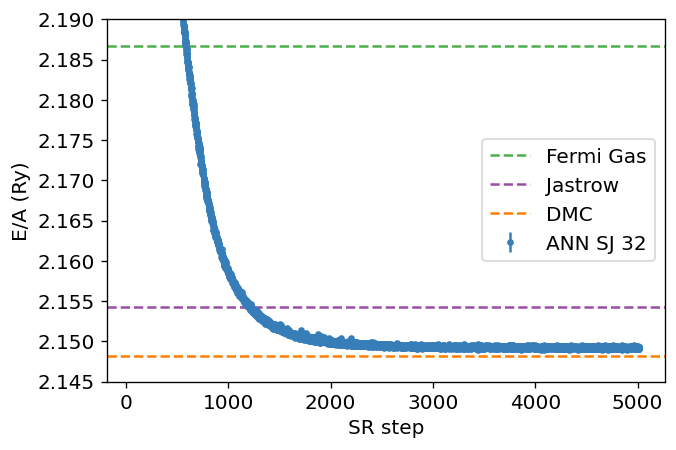
\includegraphics[width=0.9\linewidth]{figures/elgasnew.png}}

\vspace{6mm}

\end{block}
\end{frame}

\begin{frame}[plain,fragile]
\frametitle{Switching to quantum dots}

The Hamiltonian of the quantum dot is given by
\[ \hat{H} = \hat{H}_0 + \hat{V}, 
\]
where $\hat{H}_0$ is the many-body HO Hamiltonian, and $\hat{V}$ is the
inter-electron Coulomb interactions. In dimensionless units,
\[ \hat{V}= \sum_{i < j}^N \frac{1}{r_{ij}},
\]
with $r_{ij}=\sqrt{\mathbf{r}_i^2 - \mathbf{r}_j^2}$.

Separable Hamiltonian with the relative motion part ($r_{ij}=r$)
\[ 
\hat{H}_r=-\nabla^2_r + \frac{1}{4}\omega^2r^2+ \frac{1}{r},
\]
Analytical solutions in two and three dimensions for two electrons (\href{{https://journals.aps.org/pra/abstract/10.1103/PhysRevA.48.3561}}{M. Taut 1993 and 1994}).
\end{frame}


\begin{frame}{Quantum Dots as Artificial Atoms}
\begin{itemize}
\item Semiconductor-confined electrons
\item Tunable confinement $\omega$
\item Strong Coulomb correlations
\item Few-body → mesoscopic regime
\end{itemize}

\vspace{0.3cm}
Goal:
\[
\text{Understand correlation-driven structure formation}
\]
\end{frame}


\begin{frame}{Why Is This Hard?}
\begin{itemize}
\item Exponential Hilbert space growth
\item Strong correlation effects
\item Near-Wigner crystallization at weak confinement
\end{itemize}

Traditional methods:
\begin{itemize}
\item Exact diagonalization (small $N$)
\item Diffusion Monte Carlo
\item Configuration interaction
\end{itemize}
\end{frame}

\begin{frame}{Idea of Physics-Informed Neural Networks (PINNs)}
Instead of sampling:
\[
H\Psi = E\Psi
\]

Minimize PDE residual:
\[
\mathcal{L}
=
\langle |(H-E)\Psi_\theta|^2 \rangle
\]

Advantages:
\begin{itemize}
\item No stochastic Monte Carlo noise
\item Direct enforcement of Schrödinger equation
\item Continuous representation
\end{itemize}
See demonstration of PINNs at \url{https://github.com/CompPhysics/AdvancedMachineLearning/blob/main/doc/pub/week3/ipynb/BlackScholesPINN.ipynb}
\end{frame}

\begin{frame}{Wavefunction Ansatz}
\[
\Psi(R)
=
\text{SD}(R')
\exp(U(R) + W_\theta(R))
\]

Components:
\begin{itemize}
\item Slater determinant
\item Jastrow correlation
\item Neural correlator
\item Backflow
\item Permutation invariant construction
\end{itemize}
\end{frame}

\begin{frame}[plain,fragile]
\frametitle{What is backflow?}
\begin{alertblock}{Learned nonlocal transformations of coordinates}
Backflow in neural quantum state calculations is a learned, nonlocal
transformation of particle coordinates or features that allows the
wavefunction to encode collective many-body correlations and accurate
fermionic nodal structures far beyond mean-field or Jastrow forms.
\end{alertblock}
\begin{alertblock}{CTNN backflow}

CTNN backflow is a symmetry-preserving, convolutional realization of
backflow in neural quantum states, where effective coordinates or
features are generated by translation-invariant neural networks to
encode collective many-body correlations and improve fermionic nodal
structure efficiently.
\end{alertblock}

\end{frame}



\begin{frame}[plain,fragile]
\frametitle{PINNs and harmonic oscillator quantum dot}

%\begin{table*}[t]
\footnotesize{
  \centering
%  \begin{threeparttable}
    \begin{tabular}{c|c|c|cc|cc}
      $N$ & $\omega$ & DMC & PINN+BF & \%\,err & PINN+CTNN & \%\,err \\
      2 & 0.001 & --- & $0.0137948(8)$ & --- & $\mathbf{0.013778(1)}$ & --- \\
    & 0.01 & ---            & $0.69125(2)$  & --- & $\mathbf{0.69036(1)}$ & --- \\
    & 0.10 & $3.55385(5)$   & $3.5549(1)$   & $+0.0295$ & $\mathbf{3.55388(5)}$ & $+0.0008$ \\
    & 0.50 & $11.78484(6)$  & $11.7895(4)$  & $+0.0395$  & $\mathbf{11.7847(2)}$ & $-0.0000$ \\
    & 1.00 & $20.15932(8)$  & $20.1610(6)$  & $+0.0083$  & $\mathbf{20.1585(3)}$ & $-0.0041$ \\
    12 & 0.001 & ---          & $0.515823(3)$ & --- & $\mathbf{0.515365(4)}$ & --- \\
    & 0.01 & ---           & $2.48620(5)$  & --- & $\mathbf{2.47363(4)}$ & --- \\
    & 0.10 & $12.26984(8)$ & $12.2731(2)$  & $+0.0160$ & $\mathbf{12.2718(1)}$ & --- \\
    & 0.50 & $39.1596(1)$  & $39.1786(8)$  & $+0.0485$ & $\mathbf{39.1604(3)}$ & $+0.0018$ \\
    & 1.00 & $65.7001(1)$  & $65.717(1)$   & $+0.0257$ & $\mathbf{65.69556(5)}$ & $-0.0069$ \\
    20 & 0.001 & ---          & --- & --- & $\mathbf{1.293033(6)}$ & --- \\
    & 0.01 & ---           & ---  & --- & $\mathbf{6.14645(5)}$ & --- \\
    & 0.10 & $29.9779(1)$ & ---  & --- & $29.9888(2)$ & $+0.0364$ \\
    & 0.50 & $93.8752(1)$  & ---  & --- & $\mathbf{93.8789(5)}$ & $+0.0040$ \\
    & 1.00 & $155.8822(1)$  & ---   & --- & $\mathbf{155.8738(7)}$ & $-0.0024$ \\
\end{tabular}
%\end{threeparttable}
%\end{table*}}
}

\end{frame}








\begin{frame}[plain,fragile]
\frametitle{Observations (or conclusions if you prefer)}

\begin{block}{}
\begin{itemize}
\item Need for AI/Machine Learning in physics, lots of ongoing activities

\item To solve many complex problems and facilitate discoveries, multidisciplinary efforts efforts are required involving scientists in  physics, statistics, computational science, applied math and other fields.

\item There is a need for  focused AI/ML learning efforts that will benefit accelerator science and experimental and theoretical programs
\end{itemize}

\noindent
\end{block}
\end{frame}

\begin{frame}[plain,fragile]
\frametitle{More observations}

\begin{block}{}
\begin{itemize}
\item How do we develop insights, competences, knowledge in statistical learning that can advance a given field?
\begin{itemize}

  \item For example: Can we use ML to find out which correlations are relevant and thereby diminish the dimensionality problem in standard many-body  theories?

  \item Can we use AI/ML in detector analysis, experimental design, analysis of experimental data and more?

  \item Can we use AL/ML to carry out reliable extrapolations by using current experimental knowledge and current theoretical models?

\end{itemize}

\noindent
\item The community needs to invest in relevant educational efforts and training of scientists with knowledge in AI/ML. These are great challenges to the CS and DS communities

\item Quantum computing and quantum machine learning not discussed here

\item Most likely tons of things I have forgotten
\end{itemize}

\noindent
\end{block}
\end{frame}

\begin{frame}[plain,fragile]
\frametitle{Possible start to raise awareness about ML in our own field}

\begin{block}{}
\begin{itemize}
\item Make an ML challenge in your own field a la \href{{https://home.cern/news/news/computing/higgs-boson-machine-learning-challenge}}{Learning to discover: the Higgs boson machine learning challenge}. Alternatively go to kaggle.com at \href{{https://www.kaggle.com/c/higgs-boson}}{\nolinkurl{https://www.kaggle.com/c/higgs-boson}}

\item HEP@CERN and HEP in general have made significant impacts in the field of machine learning and AI. Something to learn from
\end{itemize}

\noindent
\end{block}
\end{frame}


\end{document}



